\documentclass[12pt]{extreport} % Schriftgröße: 8pt, 9pt, 10pt, 11pt, 12pt, 14pt, 17pt oder 20pt

% Language Setup (Deutsch)
\usepackage[utf8]{inputenc} 
\usepackage[english]{babel}

%% Packages
\usepackage{scrextend}
\usepackage{amssymb}
\usepackage{amsthm}
\usepackage{amsmath}
\usepackage[inline]{enumitem}
\usepackage{changes}
\usepackage{chngcntr}
\usepackage{cmap}
\usepackage{color}
\usepackage{csquotes}
\usepackage{float}
\usepackage{hyperref}
\usepackage{footnote}
\usepackage{lmodern}
\usepackage{makeidx}
\usepackage{mathtools} 
\usepackage{xpatch}
\usepackage{pgfplots}
\usepackage{stmaryrd}
\usepackage{pbox}
\usepackage{apptools}
\usepackage{booktabs}
\usepackage{dsfont}
\usepackage{subcaption}
	\expandafter\def\csname ver@subfig.sty\endcsname{}
\usepackage{graphicx}
\usepackage{mathrsfs}
\usepackage[square,numbers]{natbib}
\usepackage{nicefrac}
\usepackage{pgf}
\usepackage{pgfplots}
\usepackage{tikz}
\usepackage{tocloft}
\usepackage{url}
\usepackage{xpatch}
\usepackage{microtype}
\usepackage{pgfplots}
\usepackage{minibox}
\usepackage{xcolor}
\usepackage{sgame}  % Game theory packages
\usepackage{subfig} % Manipulation and reference of small or sub figures and tables

\makesavenoteenv{tabular}
\usepgfplotslibrary{fillbetween}
\usetikzlibrary{patterns}
\usetikzlibrary{decorations.markings}
\usetikzlibrary{calc, intersections}
\usetikzlibrary{trees, calc} % For extensive form games
\pgfplotsset{compat=1.7}
\usetikzlibrary{calc}	
\usetikzlibrary{matrix}	

\usepgfplotslibrary{fillbetween}
\usetikzlibrary{patterns}
\usetikzlibrary{decorations.markings}
\usetikzlibrary{calc, intersections}
\usetikzlibrary{trees, calc} % For extensive form games
\pgfplotsset{compat=1.7}
\usetikzlibrary{calc}	
\usetikzlibrary{matrix}	

% Options
\makeatletter%%  
  % Linkfarbe, {0,0.35,0.35} für Türkis, {0,0,0} für Schwarz 
  \definecolor{linkcolor}{rgb}{0,0.35,0.35}
  % Zeilenabstand für bessere Leserlichkeit
  \def\mystretch{1.75} 
  % Publisher definieren
  \newcommand\publishers[1]{\newcommand\@publishers{#1}} 
  % Enumerate im 1. Level: \alph für a), b), \dotsc
  \renewcommand{\labelenumi}{\alph{enumi})} 
  % Enumerate im 2. Level: \roman für (i), (ii), \dotsc
  \renewcommand{\labelenumii}{(\roman{enumii})}
  % Zeileneinrückung am Anfang des Absatzes
  \setlength{\parindent}{0pt} 
  % Verweise auf Enumerate, z.B.: 3.2 a)
  \setlist[enumerate,1]{ref={\thesatz ~ \alph*)}}
  % Für das Proof-Environment: 'Beweis:' anstatt 'Beweis.'
  \xpatchcmd{\proof}{\@addpunct{.}}{\@addpunct{:}}{}{} 
  % Nummerierung der Bilder, z.B.: Abbildung 4.1
  \@ifundefined{thechapter}{}{\def\thefigure{\thechapter.\arabic{figure}}} 
\makeatother%

% Meta Setup (Für Titelblatt und Metadaten im PDF)
\title{Advanced Game Thoery}
\author{Prof. Dr. Clemens Puppe}
\date{Vorlesungsmitschrieb ~\vspace{0.2cm} \\ Wintersemester 2016/17}
\publishers{Karlsruher Institut für Technologie}

%% Math. Definitions
\newcommand{\C}{\mathbb{C}}
\newcommand{\N}{\mathbb{N}}
\newcommand{\Q}{\mathbb{Q}}
\newcommand{\R}{\mathbb{R}}
\newcommand{\Z}{\mathbb{Z}}

%% Theorems (unnamedtheorem = Theorem ohne Namen)
\newtheoremstyle{named}{}{}{\normalfont}{}{\bfseries}{:}{0.25em}{#2 \thmnote{#3}}
\newtheoremstyle{itshape}{}{}{\itshape}{}{\bfseries}{:}{ }{}
\newtheoremstyle{normal}{}{}{\normalfont}{}{\bfseries}{:}{ }{}
\renewcommand*{\qed}{\hfill\ensuremath{\square}}

\theoremstyle{named}
\newtheorem{unnamedtheorem}{Theorem} \counterwithin{unnamedtheorem}{chapter}
\newtheorem*{unnamedtheorem*}{Theorem} 

\theoremstyle{itshape}
\newtheorem{theorem}[unnamedtheorem]{Theorem}	
\newtheorem{satz}[unnamedtheorem]{Satz}	
\newtheorem*{definition}{Definition}

\theoremstyle{normal}
\newtheorem{beispiel}[unnamedtheorem]{Beispiel}
\newtheorem{example}[unnamedtheorem]{Example}
\newtheorem{folgerung}[unnamedtheorem]{Folgerung}
\newtheorem{hilfssatz}[unnamedtheorem]{Hilfssatz}
\newtheorem{lemma}[unnamedtheorem]{Lemma}
\newtheorem{proposition}[unnamedtheorem]{Proposition}
\newtheorem{anwendung}[unnamedtheorem]{Anwendung}
\newtheorem{anwendungen}[unnamedtheorem]{Anwendungen}
\newtheorem*{beispiel*}{Beispiel}
\newtheorem*{example*}{Example}
\newtheorem*{beispiele}{Beispiele}
\newtheorem*{examples}{Examples}
\newtheorem*{bemerkung}{Bemerkung} 
\newtheorem*{comment*}{Comment} 
\newtheorem*{bemerkungen}{Bemerkungen}
\newtheorem*{bezeichnung}{Bezeichnung}
\newtheorem*{eigenschaften}{Eigenschaften}
\newtheorem*{erinnerung}{Erinnerung}
\newtheorem*{folgerung*}{Folgerung}
\newtheorem*{folgerungen}{Folgerungen}
\newtheorem*{hilfssatz*}{Hilfssatz}
\newtheorem*{regeln}{Regeln}
\newtheorem*{schreibweise}{Schreibweise}
\newtheorem*{schreibweisen}{Schreibweisen}
\newtheorem*{uebung}{übung}
\newtheorem*{vereinbarung}{Vereinbarung}

%% Template
\makeatletter%
\DeclareUnicodeCharacter{00A0}{ } \pgfplotsset{compat=1.7} \hypersetup{colorlinks,breaklinks, urlcolor=linkcolor, linkcolor=linkcolor, pdftitle=\@title, pdfauthor=\@author, pdfsubject=\@title, pdfcreator=\@publishers}\DeclareOption*{\PassOptionsToClass{\CurrentOption}{report}} \ProcessOptions \def\baselinestretch{\mystretch} \setlength{\oddsidemargin}{0.125in} \setlength{\evensidemargin}{0.125in} \setlength{\topmargin}{0.5in} \setlength{\textwidth}{6.25in} \setlength{\textheight}{8in} \addtolength{\topmargin}{-\headheight} \addtolength{\topmargin}{-\headsep} \def\pulldownheader{ \addtolength{\topmargin}{\headheight} \addtolength{\topmargin}{\headsep} \addtolength{\textheight}{-\headheight} \addtolength{\textheight}{-\headsep} } \def\pullupfooter{ \addtolength{\textheight}{-\footskip} } \def\ps@headings{\let\@mkboth\markboth \def\@oddfoot{} \def\@evenfoot{} \def\@oddhead{\hbox {}\sl \rightmark \hfil \rm\thepage} \def\chaptermark##1{\markright {\uppercase{\ifnum \c@secnumdepth >\m@ne \@chapapp\ \thechapter. \ \fi ##1}}} \pulldownheader } \def\ps@myheadings{\let\@mkboth\@gobbletwo \def\@oddfoot{} \def\@evenfoot{} \def\sectionmark##1{} \def\subsectionmark##1{}  \def\@evenhead{\rm \thepage\hfil\sl\leftmark\hbox {}} \def\@oddhead{\hbox{}\sl\rightmark \hfil \rm\thepage} \pulldownheader }	\def\chapter{\cleardoublepage  \thispagestyle{plain} \global\@topnum\z@ \@afterindentfalse \secdef\@chapter\@schapter} \def\@makeschapterhead#1{ {\parindent \z@ \raggedright \normalfont \interlinepenalty\@M \Huge \bfseries  #1\par\nobreak \vskip 40\p@ }} \newcommand{\indexsection}{chapter} \patchcmd{\@makechapterhead}{\vspace*{50\p@}}{}{}{}
	% Titlepage
	\def\maketitle{ \begin{titlepage} 
			~\vspace{3cm} 
		\begin{center} {\Huge \@title} \end{center} 
	 		\vspace*{1cm} 
	 	\begin{center} {\large \@author} \end{center} 
	 	\begin{center} \@date \end{center} 
	 		\vspace*{7cm} 
	 	\begin{center} \@publishers \end{center} 
	 		\vfill 
	\end{titlepage} }
\makeatother%

% Indexdatei erstellen
\makeindex 

\begin{document}

\pagenumbering{Alph}
\begin{titlepage}
	\maketitle
	\thispagestyle{empty}
\end{titlepage}
\pagenumbering{arabic}
	
% Inhaltsverzeichnis
\tableofcontents
\thispagestyle{empty} 
  
% Skript - Anfang 
\chapter{Noncooperative Games}

\section{Basic Elements of Noncooperative Games}


\begin{definition}
	A \textbf{game} is a formal representation of a situation in which a number of individuals interact in a setting of strategic interdependence.
	
	\begin{itemize}
		\item The players: Who is involved?
		\item The rules: Who moves when? What do they know when they move? What can they do?
		\item The outcomes: For each possible set of actions by the players, what is the outcome of the game?
		\item The payoffs: What are the players' preferences over the possible outcomes?
	\end{itemize} 
\end{definition} ~\newpage


\begin{example}[of simultaneous move games]  ~\
	\begin{enumerate}
		\item Matching Pennies
			\begin{figure}[h!] \centering
  				\begin{game}{2}{2}[Player $1$][Player $2$]
   	    			   	 	&	  Heads    &  Tails   \\
   	 				Heads   &    $-1, 1$   & $1, -1$  \\
   	 				Tails   &    $1, -1$   & $-1, 1$  \\
   				\end{game}
			\end{figure} 
		\item Meeting in New York ~\\
			\begin{figure}[H] \centering
  				\begin{game}{2}{2}[Player $1$][Player $2$]
   	    			   	 		&	Empire State    &  Grand Central   \\
   	 				Empire State   &    $100, 100$   & $0, 0$  \\
   	 				Grand Central   &    $0,0$   & $100, 100$  \\
   				\end{game}
			\end{figure}
		\item Examples of (simple) dynamic games
			 \begin{figure}[h!]
 	\centering
	\caption*{Prisoner's Dilemma in Extensive-form \label{PDExtensive}}
    \begin{tikzpicture}[thin,
      level 1/.style={sibling distance=40mm},
      level 2/.style={sibling distance=25mm},
      level 3/.style={sibling distance=15mm},
      every circle node/.style={minimum size=1.5mm,inner sep=0mm}]
      
      \node[circle,draw,label=above:$P_1$] (root) {}
        child { node [circle,fill,label=above:$P_2$] {}
          child { 
            node {$($-$1,1)$}
            edge from parent
              node[left] {$H$}}
          child { 
            node {$(1,$-$1)$}
            edge from parent
              node[right] {$T$}}
          edge from parent
            node[left] {$H$}}
        child { node [circle,fill,label=above:$P_{2}$] {}
          child { 
            node {$(1,$-$1)$}
              edge from parent
                node[left] {$H$}}
          child { 
            node {$($-$1,1)$}
              edge from parent
                node[right] {$T$}}
           edge from parent
             node[right] {$T$}};
    \end{tikzpicture}
  \end{figure}
		\item Matching Pennies Version C ~\\
	% Node styles
	\tikzset{
	% Two node styles for game trees: solid and hollow
	solid node/.style={circle,draw,inner sep=1.5,fill=black},
	hollow node/.style={circle,draw,inner sep=1.5}
	} 

\begin{figure}[h!]
	\centering
	\begin{tikzpicture}[scale=1.5,font=\footnotesize]
	% Specify spacing for each level of the tree
	\tikzstyle{level 1}=[level distance=15mm,sibling distance=40mm]
	\tikzstyle{level 2}=[level distance=15mm,sibling distance=22mm]
	\tikzstyle{level 3}=[level distance=15mm,sibling distance=15mm]
	% The Tree
	\node(0)[hollow node,label=above:{$P1$}]{}
	child{node(1)[solid node]{}
		child{node[label=below:{$($-$1,1)$}]{} edge from parent node[left]{$H$}}
		child{node(3)[label=below:{$(1,$-$1)$}]{} edge from parent node[right]{$T$}}
		edge from parent node[left,xshift=-3]{$H$}
	}
	child{node(2)[solid node]{}
		child{node[label=below:{$(1,$-$1)$}]{} edge from parent node[left]{$H$}}
		child{node[label=below:{$($-$1,1)$}]{} edge from parent node[right]{$T$}}
		edge from parent node[right,xshift=3]{$T$}
	};
	% information set
	\draw[dashed,rounded corners=10]($(1) + (-.2,.25)$)rectangle($(2) +(.2,-.25)$);
	% specify mover at 2nd information set
	\node at ($(1)!.5!(2)$) {$P2$};
	\end{tikzpicture}
\end{figure}

	\end{enumerate}
\end{example} ~\

\begin{definition}[Information] ~\
	\begin{enumerate}
		\item \textbf{Information Set:} A player doesn't know which of the nodes in the information set she is actually at. Therefore, at any decision node in a player's information set, there must be the same possible actions. More formally,in the extensive form, an information set is a set of decision nodes such that:
			\begin{enumerate}
				\item Every node in the set belongs to one player.
			 	\item When play reaches the information set, the player with the move cannot differentiate between nodes within the information set, i.e. if the information set contains more than one node, the player to whom that set belongs does not know which node in the set has been reached.
			 			\end{enumerate}
			Therefore, at any decision node in a player's information set, there must be the same possible actions.
		\item \textbf{Perfect Information:} A game is said to be of perfect information if each information set contains a single decision node. Otherwise, it is a game of \textbf{imperfect information}. In other words, perfect information persists, if each player, when making any decision, is perfectly informed of all the events that have previously occurred, including the early equipment.
	\end{enumerate}
\end{definition} 

\begin{definition}[Extensive Form Game] ~\
	A game in \textbf{extensive form} consists of:
	\begin{enumerate}[label=(\roman*\upshape)]
		\item A finite set of nodes $\mathcal{X}$, a finite set of possible actions $\mathcal{A}$, and a finite set of players $\{1, \dotsc, l\}$.
		\item A funktion $p \colon \mathcal{X} \rightarrow \{ \mathcal{X} \cup \emptyset \}$ specifying a single immediate predecessor of each node $x$; $p(x) \in \mathcal{X}$ expect for one element $x_{0}$, the \textbf{initial node}. The immediate \textbf{successor node} of $x$ are $s(x) = p^{-1}(x)$. ~\\
			To have a tree structure, a predecessor can never be a successor and vice versa. The set of \textbf{terminal nodes} $T = \{ x \in \mathcal{X} \colon s(x) = \emptyset \}$. All other nodes $X \setminus T$ are \textbf{decision nodes}.
		\item A function $\alpha \colon \mathcal{X} \setminus \{ x_{0} \} \rightarrow \mathcal{A}$ giving the action that leads to any non-initial node $x$ from its immediate predecessor $p(x)$ with $x', x'' \in s(x); x' \neq x'' \Rightarrow \alpha(x') \neq \alpha(x'')$. The set of choices at decision node $x$ is $c(x) = \{ a \in \mathcal{A} \colon a = \alpha(x') \text{ for some } x' \in s(x) \}$.
		\item A collection of information sets $\mathcal{H}$, and a function $H \colon \mathcal{X} \rightarrow \mathcal{H}$ assigning each decision node $x$ to an information set $H(x) \in \mathcal{H}$ with $c(x) = c(x')$ if H(x) = $H(x')$. ~\\
			The choices available at information set $H$ can be written as
			$$ C(H) = \{ a \in \mathcal{A} \colon a \in c(x) \text{ for } x \in H \}. $$
		\item A function $\iota \colon \mathcal{H} \rightarrow \{ 0, 1, \dotsc, l \}$ assigning a player to each information set ($i = 0$ 'nature'). The collection of player i's information set is denoted by
			$$ \mathcal{H}_i = \{ H \in \mathcal{H} \colon i = \iota(H) \}. $$
		\item A function $\rho \colon \mathcal{H}_0 \times \mathcal{A} \rightarrow [0,1]$ assigning a probability to each action of nature with $\rho(H,a) = 0$ if $a \notin C(H)$ und $\sum_{a \in C(H)} \rho(H, a) = 1$ for all $H \in \mathcal{H}_{0}$.
		\item A collection of payoff function $u = \{ u_1(\cdot), \dotsc, u_l(\cdot) \}$, where $u_i \colon T \rightarrow \R$.
	\end{enumerate}
	\textbf{A game in extensive form:} $\Gamma_E = \{ \mathcal{X}, \mathcal{A}, I, p(\cdot), \alpha(\cdot), \mathcal{H}, H(\cdot), \iota(\cdot), \rho(\cdot), u \}$.
\end{definition}

\begin{comment*}
	Restrictions of this definition:
	\begin{enumerate}
		\item Finite set of actions
		\item Finite number of moves
		\item Finite number 	of players
	\end{enumerate}
\end{comment*}

\begin{definition}[Strategy]
	Let $\mathcal{H}_i$ denote the collection of player $i$'s information sets, $\mathcal{A}$ the set of possible actions in the game, and $C(H) \subset \mathcal{A}$ the set of actions possible at information set $H$. A \textbf{strategy} for player $i$ is a function $s_i \colon \mathcal{H}_i \Rightarrow \mathcal{A}$ such that $s_i(H) \in C(H)$ for all $H \in \mathcal{H}_i$.
\end{definition} 

\begin{definition}[Normal Form Representation]
	For a game with $I$ players, the \textbf{normal form representation} $\Gamma_N$ specifies for each player $i$ a set of strategies $\mathcal{S}_{i}$ (with $s_i \in \mathcal{S}_i$) and a payoff function $u_i(s_1, \dotsc, s_l)$, formally 
	$$ \Gamma_N = \left[I, \{ S_i \}, \{ u_i(\cdot) \} \right]. $$
\end{definition} 

\begin{definition} ~\
	\begin{enumerate}
		\item $s_i \colon \mathcal{H}_i \rightarrow \mathcal{A}$ describes deterministic choices at each $H \in \mathcal{H}_i$ and is called a \textbf{pure strategy}
		\item a \textbf{mixed strategy} is a probability distribution over all pure strategies $\sigma_i \colon \mathcal{S}_i \rightarrow [0, 1]$, with $\sigma_i(s_i) \geq 0$ and $\sum_{s_i \in \mathcal{S}_i} \sigma_i(s_i) = 1$.
		\item player $i$'s set of possible mixed strategies can be associated with the points of the simplex $\Delta(\mathcal{S}_i)$, called the \textbf{mixed extension} of $\mathcal{S}_i$.
		\item since we assume that individuals are expected utility maximisers, player $i$'s utility of a profile of mixed strategies $\sigma = \left( \sigma_i, \dotsc, \sigma_l \right)$ is given by
			$$ u_i(\sigma) = \sum_{s \in \mathcal{S}} [\sigma_1(s_1) \cdot \sigma_2(s_2) \cdot \dotsc \cdot \sigma_l(s_l)] \cdot u_i(s), $$
			where $s = (s_1, \dotsc, s_l)$.
	\end{enumerate}
\end{definition}

\begin{definition}[Behaviour Strategy]
	Given an extensive form game $\Gamma_E$, a \textbf{behaviour strategy} for player $i$ specifies for every information set $H \in \mathcal{H}_i$ and action $a \in C(H)$, a probability $\lambda_i(a, H) \geq 0$, with
	$$ \sum_{a \in C(H)} \lambda_i(a, H) = 1 \text{ for all } H \in \mathcal{H}_i. $$
\end{definition}

\begin{definition}[Perfect Recall]
	A player has \textbf{perfect recall} if he doesn't \enquote{forget} what she once knew, including her own actions. That means, perfect recall refers to the assumption that, at every decision node, each Player remembers what he did in prior moves, and each player remembers everything that he knew before; effectively, the assumption is one that players never forget information once it is acquired.
\end{definition}

\begin{theorem}
	If $\Gamma_E$ is an extensive form game with perfect recall, then for any mixed strategy there is an outcome equivalent behaviour strategy and vice versa.	
\end{theorem}

\section{Rationalisable Strategies}

Central question of Game Theory: What should we expect to observe in a game played by rational players? Or more precisely: What should we expect to observe in a game played by rational players who are fully knowledgeable about the structure of the game and each others' rationality? ~\\

We first address the above question for simultaneous-move games, which we study using their normal form representation. We use the following notation:
\begin{itemize}
	\item $\Gamma_N = \left[I, \{ S_i \}, \{ u_i(\cdot) \right]$ if we consider pure strategies only, ~\\
		$\Gamma_{N} = \left[I, \{ \Delta(S_i)\}, \{ u_i(\cdot) \} \right]$ if we allow for mixed strategies
	\item $s_{-i} = (s_1, \dotsc, s_{i-1}, s_{i+1}, \dotsc, s_l) \in \mathcal{S}_{-i}$ where $\mathcal{S}_{-i} = S_1 \times \dotsc \times S_{i-1} \times S_{i+1} \times \cdots \times S_{l}$
	\item $s = (s_i, s_{-i})$
\end{itemize}

\begin{example}[Prisoners' Dilemma] ~\\
			\begin{figure}[h!] \centering
  				\begin{game}{2}{2}[Player $1$][Player $2$]
   	    			   	 	&	  don't confess    &  confess   \\
   	 				don't confess   &    $-2, -2$   & $-10, -1$  \\
   	 				confess   &    $-1, -10$   & $-5, -5$  \\
   				\end{game}
			\end{figure}
\end{example}

What should we expect to observe in the Prisoners' Dilemma?

\begin{definition}[Strictly Dominant Strategy]
	A strategy $s_i \in \mathcal{S}_i$ is \textbf{strictly dominant} for player $i$ in game $\Gamma_N = \left[I, \{  \mathcal{S}_i \}, \{ u_i(\cdot)\} \right]$ if for all $s_i' \neq s_i$:
	$$ u_{i}(s_i, s_{-i}) > u_i(s_i', s_{-i})  $$
	for all $s_{i} \in \mathcal{S}_{-i}$.
\end{definition}
Applied to Prisoner's Dilemma: Confess is a strictly dominant strategy for each player.

\begin{definition}[Strictly Dominated Strategy]
	$s_i \in \mathcal{S}_i$ is \textbf{strictly dominated} for player $i$ in game $\Gamma_N$ if there exists another strategy $s_i' \in \mathcal{S}_i$ such that:
	$$ u_i(s_i', s_{-i}) > u_i(s_i, s_{-i}) $$
	for all $s_{-i} \in \mathcal{S}_{-i}$. In this case we say that $s_i'$ strictly dominates $s_i$.
\end{definition}


\begin{definition}[Weakly Dominated Strategy]
	$s_i \in \mathcal{S}_{i}$ is \textbf{weakly dominated} for player $i$ in game $\Gamma_N$ if there exists another strategy $s_i' \in \mathcal{S}_i$ such that:
	$$ u_i(s_i', s_{-i}) \geq u_i(s_i, s_{-i}) $$
	for all $s_{-i} \in \mathcal{S}_{-i}$, with strict inequality for at least one $s_{-i}$.
\end{definition} 

\begin{example} ~\\
	\begin{figure}[h!] \centering
		\begin{subfigure}{.5\textwidth} \centering
  				\begin{game}{3}{2}[Player $1$][Player $2$]
   	    			   	 	&	  L    &  R   \\
   	 				U   &    $1, -1$   & $-1, 1$  \\
   	 				M   &    $-1, 1$   & $1, -1$  \\
   					D   &    $-2, 5$   & $-3, 2$  \\
   				\end{game} $$ \Rightarrow D \text{ is strictly dominated by } U \text{ and } M.$$
		\end{subfigure}%
		\begin{subfigure}{.5\textwidth} \centering	
   				\begin{game}{3}{2}[Player $1$][Player $2$]
   	    			   	 	&	  L    &  R   \\
   	 				U   &    $5, 1$   & $4, 0$  \\
   	 				M   &    $6, 0$   & $3, 1$  \\
   					D   &    $6,4$   & $4, 4$  \\
   				\end{game} $$\Rightarrow U \text{ and } M \text{ are weakly dominated by } D.$$
		\end{subfigure}
	\end{figure}
\end{example} 

\begin{example}[Prisoners’ Dilemma – A Variation]
	Assume Prisoner 1 is the district attorney’s brother: If neither player confesses, player 1 is free	 ~\\
	\begin{figure}[h!] \centering
  				\begin{game}{2}{2}[Player $1$][Player $2$]
   	    			   	 	&	  don't confess    &  confess   \\
   	 				don't confess   &    $0, -2$   & $-10, -1$  \\
   	 				confess   &    $-1, -10$   & $-5, -5$  
   	   				\end{game}
	\end{figure}
	$$\Rightarrow \text{ Player 1 has no dominant strategy anymore}.$$
\end{example}

In this game, the iterated elimination of strictly dominated strategies still leads to a unique prediction. In general, the order of elimination of strictly dominated strategies does not matter! How about iterated elimination of weakly dominated strategies?

\begin{definition}
	A strategy $\sigma_i \in \Delta(\mathcal{S}_i)$ is strictly dominated for $i$ in game $\Gamma_{N} = [I, \{ \Delta(\mathcal{S}_i)\}, \{ u_i(\cdot) \}]$ if there exists another strategy $\sigma_i' \in \Delta(\mathcal{S}_i)$ such that for all $\sigma_{-i} \in \Pi_{j \neq i} \Delta(\mathcal{S}_{j})$:
	$$ u_{i}(\sigma_i', \sigma_{-i}) > u_i(\sigma_i, \sigma_{-i}). $$
\end{definition}


\begin{proposition}
	Player $i$'s pure strategy $s_i \in \mathcal{S}_i$ is strictly dominated in a game $\Gamma_N = [I, \{ \Delta(\mathcal{S}_i)\}, \{ u_i(\cdot)\}]$ if and only if there exists another strategy $\sigma_i' \in \Delta(\mathcal{S}_i)$ such that
	$$ u_i(\sigma_i', s_{-i}) > u_i(s_i, s_{-i}) \text{ for all } s_{-i} \in \mathcal{S}_{-i}. $$
	
	\begin{proof}
		This follows because we can write
		$$ u_i(\sigma_i', \sigma_{-i}) - u_i(s_i, \sigma_{-i}) = \sum_{s_{-i} \in \mathcal{S}_{-i}} \left[ \Pi_{k \neq i} \sigma_{k}(s_{k}) \right] \left[ u_{i}(\sigma_i', s_{-i}) - u_{i}(s_i, s_{-i}) \right]. $$
		And this expression is positive for all $\sigma_{-i}$ if and only if $u_i(\sigma_i', s_{-i}) - u_{i}(s_{i}, s_{-i})$ is positive for all $s_{-i}$.
	\end{proof}
\end{proposition}

\begin{example} ~\
	\begin{figure}[h!] \centering
  				\begin{game}{3}{2}[Player $1$][Player $2$]
   	    			   	 	&	  L    &  R   \\
   	 				U   &    $10, 1$   & $0, 4$  \\
   	 				M   &    $4, 2$   & $4, 3$ \\
   	 				D   &    $0, 5$   & $10, 2$  

   	   				\end{game} $$\Rightarrow \frac{1}{2}U+ \frac{1}{2} D \text{ strictly dominates } M.$$
	\end{figure}
\end{example}

\begin{definition}[Best response]
	The strategy $\sigma_i$ is a \textbf{best response} for player $i$ to her rivals' strategies $\sigma_{-i}$ if:
	$$ u_i(\sigma_i, \sigma_{-i}) \geq u_i(\sigma_i', \sigma_{-i}) $$
	for all $\sigma_i' \in \Delta(\mathcal{S}_i)$. Strategy $\sigma_i$ is never a best response if there is no $\sigma_{-i}$ for which $\sigma_{i}$ is a best response.
\end{definition}

\begin{definition}[Rationalisable Strategies]
	In game $\Gamma_N = \left[I, \{ \Delta(\mathcal{S}_i) \}, \{ u_i(\cdot) \}\right]$, the strategies in $\Delta(\mathcal{S}_i)$ that survive the iterated elimination of strategies that are never a best response are known as player $i$'s \textbf{rationalisable strategies}.
\end{definition}

\begin{example} ~\\
		\begin{figure}[h!] \centering
  				\begin{game}{4}{4}[Player $1$][Player $2$]
   	    			   	 	& $b_1$ & $b_2$ & $b_3$ & $b_4$   \\
   	 				$a_1$   &    $0, \underline{7}$   & $2, 5$&    $\underline{7}, 0$   & $0, 1$  \\
   	 				$a_2$   &    $5, 2$   & $\underline{3}, \underline{3}$&    $5, 2$   & $0, 1$ \\
   	 				$a_3$   &    $\underline{7}, 0$   & $2, 5$ &    $0, \underline{7}$   & $0, 1$  \\
					$a_4$   &    $0, \underline{0}$   & $0, -2$ &    $0, \underline{0}$   & $\underline{10}, -1$ 
   	   				\end{game} $$\Rightarrow \frac{1}{2}U+ \frac{1}{2} D \text{ strictly dominates } M.$$
	\end{figure} ~\\
	$\Rightarrow b_4$ is never best response for player 2 and \textit{then} $a_4$ is never best response for player 1. ~\\
	$\Rightarrow \{a_1, a_2, a_3\}$ and $\{ b_1, b_2, b_3 \}$ are the rationalisable strategies in this game.
\end{example}

\section{Nash Equilibrium}

\begin{example}
		\begin{figure}[h!] \centering
  				\begin{game}{3}{3}[Player $1$][Player $2$]
   	    			   	 	& $L$ & $M$ & $R$   \\
   	 				$U$   &    $5, 3$   & $0, 4$&    $3,5$  \\
   	 				$M$   &    $4, 0$   & $\underline{5}, \underline{5}$&    $4, 0$ \\
   	 				$D$   &    $3, 5$   & $0, 4$ &    $5, 3$ 
   	   				\end{game}
	\end{figure} ~\\
	All strategies in this game are rationalisable, i.e. best responses to reasonable conjectures about other players' strategies. Yet only one strategy profile (namely $(M,M)$) contains best responses to correct conjectures about other players' strategies.
\end{example}


\begin{definition}[Nash Equilibrium]
	A strategy profile $s = (s_1, \dotsc, s_l)$ constitutes a Nash equilibrium (NE) of game $\Gamma_N$ if for every $i = 1, \dotsc, l$
	$$ u_i(s_i, s_{-i}) \geq u_i(s_i', s_{-i}) \text{ for all } s_i' \in \mathcal{S}_i $$
	In the game on the previous slide, there is only one Nash equilibrium.
\end{definition} ~\newpage

\begin{example}[Meeting in New York]
	\begin{enumerate}
		\item Part 1 
			\begin{figure}[h!] \centering
  				\begin{game}{2}{2}[Player $1$][Player $2$]
   	    			   	 	& $Empire State$ & $Grand Central$    \\
   	 				$Empire State$   &$\underline{100}, \underline{100}$& $0, 0$  \\
   	 				$Grand Central$   &    $0, 0$   & $\underline{100}, \underline{100}$ \\
   	   			\end{game} $$\Rightarrow (Empire State, Empire State) \text{ and } (Grand Central, Grand Central) \text{ are Nash equilibria.} $$
			\end{figure}
		\item Part 2
			\begin{figure}[h!] \centering
  				\begin{game}{2}{2}[Player $1$][Player $2$]
   	    			   	 	& $Empire State$ & $Grand Central$    \\
   	 				$Empire State$   &$\underline{100}, \underline{100}$& $0, 0$  \\
   	 				$Grand Central$   &    $0, 0$   & $\underline{1000}, \underline{1000}$ \\
   	   			\end{game} $$\Rightarrow \text{Again, } (Empire State, Empire State) \text{ and } (Grand Central, Grand Central) \text{ are Nash equilibria}. $$
			\end{figure} 
	\end{enumerate}
\end{example}

Why should we care about Nash equilibria? Why should players' conjecture about each other's play be correct?
\begin{enumerate}
	\item If there is a unique predict outcome to a game, it must be a Nash-Equilibrium.
	\item Thus, a \enquote{focal point} (see example part 2) can be the unique predicted outcome to a game only if it is a Nash-Equilibrium.
	\item An agreement between players is self-enforcing if it is a Nash-Equilibrium.
	\item In a repeated game, a social convention to play the game might emerge. Only a Nash-Equilibrium can be maintained as a stable convention.
\end{enumerate} 
 
\begin{definition}[Mixed Strategy Nash Equilibrium]
	A mixed strategy profile $\sigma = (\sigma_1, \dotsc, \sigma_l)$ constitutes a Nash equilibrium of game $\Gamma_N$ if for every $i=1, \dotsc, l$,
	$$ u_i(\sigma_i, \sigma_{-i}) \geq u_i(\sigma_i', \sigma_{-i}) \text{ for all } \sigma_i' \in \Delta(\mathcal{S}_i). $$
\end{definition} 
 
\begin{proposition} 
	Let $\mathcal{S}_{i}^{+} \subset \mathcal{S}$ denote the set of pure strategies that player $i$ plays with positive probability in mixed strategy profile $\sigma = (\sigma_1, \dotsc, \sigma_l)$. Strategy profile $\sigma$ is a Nash equilibrium in game $\Gamma_N$ if and only if for all $i = 1, \dotsc, l$,
	\begin{enumerate}
		\item $u_i(s_i, \sigma_{-i}) = u_i(s_i', \sigma_{-i})$ for all $s_i, s_i' \in \mathcal{S}_i^+$
		\item $u_i(s_i, \sigma_{-i}) \geq u_i(s_i', \sigma_{-i})$ for all $s_i \in \mathcal{S}_i^+$ and all $s_i' \notin \mathcal{S}_i^+$.
	\end{enumerate}
\end{proposition} 
 
\begin{example}[Meeting in New York 2]
			\begin{figure}[h!] \centering
  				\begin{game}{2}{2}[Player $1$][Player $2$]
   	    			   	 	& $Empire State$ & $Grand Central$    \\
   	 				$Empire State$   &$\underline{100}, \underline{100}$& $0, 0$  \\
   	 				$Grand Central$   &    $0, 0$   & $\underline{1000}, \underline{1000}$ \\
   	   			\end{game} $$\Rightarrow \text{Again, } (Empire State, Empire State) \text{ and } (Grand Central, Grand Central) \text{ are Nash equilibria}. $$
			\end{figure} ~\\
		There are two pure strategy Nash-Equilibria, but are there also mixe strategy Nash-Equilibria? Let $p$ denote the probability of (player $-i$) playing ES. Then for player $i$ to play ES and GC with positive probability in a Nash-Equilibrium, we need
		$$ u_i(ES, p\cdot ES + (1-p) \cdot GC) = u_i(GC, p \cdot ES + (1 - p) \cdot GC) $$
		$$ \Rightarrow 100 \cdot p = 1000 \cdot (1 - p) \iff p = \frac{10}{11} $$
		Thus, there is a mixed strategy Nash-Equilibrium with both players playing ES with probability $\frac{10}{11}$.
\end{example} 
 
\begin{itemize}
	\item In a Nash equilibrium each player's strategy is a best response to all other players' strategies.
	\item Let $b_i(s_{-i})$ denote the best response(s) of player $i$ to the strategies $s_{-i}$
	\item Then $b_i \colon \mathcal{S}_{-i} \rightarrow \mathcal{S}_i$ is a correspondence, called player $i$'s best response correspondence.
	\item Define $b \colon \mathcal{S} \rightarrow \mathcal{S}$ by $(s_1, \dotsc, s_l) \mapsto b_1(s_{-1}) \times \dotsc \times b_l(s_{-l})$
	\item A strategy profile $s \in \mathcal{S}$ is a Nash equilibrium if and only if $s \in b(s)$
	\item Thus, to prove existence of Nash equilibria, we have to show that a fixed point of the correspondence $b$ exists
	\item To do so, we employ Kakutani's fixed-point theorem
\end{itemize} 
 
\begin{lemma}
	If $\mathcal{S}_1, \dotsc, \mathcal{S}_l$ are nonempty, compact and convex and $u_i$ is continuous in $\mathcal{S}_1, \dotsc, \mathcal{S}_l$ and quasi-concave, then player $i's$ best response correspondence $b_i(\cdot)$ is nonempty-valued, convex-valued and upper hemicontinuous.
\end{lemma} 
 
\begin{definition}[Quasi-Concave Function]
	The function $f \colon A \rightarrow \mathbb{R}$, defined on the convex set $A \subset \mathbb{R}^N$, is quasi-concave if its upper contour sets $\{ x \in A \colon f(x) \geq t \}$ are convex sets.
\end{definition} 
 
\begin{definition}[Upper Hemicontinuous Correspondence]
	Given $A \subset \mathbb{R}^{N}$ and the closed set $Y \subset \mathbb{R}^{K}$, the correspondence $f \colon A \rightarrow Y$ is upper hemicontinuous if it has a closed graph and the images of compact sets are bounded.
\end{definition} 

\begin{theorem}[Kakutani's Fixed Point Theorem]
	Suppose that $A \subset \mathbb{R}^N$ is a nonempty, compact, convex set, and that $f \colon A \rightarrow A$ is a correspondence from $A$ into itself that is nonempty-valued, convex-valued and upper hemicontinuous. ~\\
	
	Then $f(\cdot)$ has a fixed point; that is, there is an $x \in A$ such that $x \in f(x)$.
\end{theorem}
 
\begin{proposition}
	A Nash equilibrium exists in game $\gamma_N$ if for all $i = 1, \dotsc, l$,
	\begin{enumerate}
		\item $\mathcal{S}_i$ is a nonempty, convex, and compact subset of some Euclidean space $\mathbb{R}^M$
		\item $u_i(s_1, \dotsc, s_l)$ is continuous in $(s_1, \dotsc, s_l)$ and quasi-concave in $s_i$.
	\end{enumerate}
	
	\begin{proof}
		By the lemma about strategy sets, $b(\cdot)$ is nonempty, convex-valued and upper hemicontinuous. By Kakutani's fixed point theorem there exists an $s \in \mathcal{S}$ such that $s \in b(s)$. By the definition of $b$: $s_i \in b_i(s_{-i})$ for all $i = 1, \dotsc, l$. Thus $s$ is a Nash equilibrium.
	\end{proof}
\end{proposition} 

\begin{proposition}
	Every Game $\Gamma_N = \left[ I, \{ \Delta(\mathcal{S}_i) \}, \{u_i(\cdot)\} \right]$ in which the sets $\mathcal{S}_1, \dotsc, \mathcal{S}_l$ have a finite number of elements has a mixed strategy Nash equilibrium.
\end{proposition}

This follows from the previous proposition on the existence of Nash equilibria because the set of mixed strategies $\Delta(\mathcal{S}_i)$ of a finite number if pure strategies is nonempty, convex, and compact.

\begin{example} ~\\
			\begin{figure}[h!] \centering
  				\begin{game}{2}{2}[Player $1$][Player $2$]
   	    			   	 	& $L$ & $R$    \\
   	 				$O$   & $-2, 1$ & $1, -1$ \\
   	 				$U$   & $1, -2$ & $-1, 1$ \\
   	   			\end{game}
			\end{figure} 
			
	\textbf{Player 1's calculation:}
	\begin{align*}
		\Rightarrow & u_1(p \cdot O + (1 - p) \cdot U, q \cdot L + (1 - q) \cdot R) \\
			& = pq (-2) + p(1-q)1 + (1-p)q1 + (1-p)(1-q)(-1) \\
			& = -2pq + p - pq + q - pq - 1 + p + q -pq \\
			& = - 5pq + 2p + 2q - 1 \\
			& = (2 - 5q)p + 2q - 1
	\end{align*}
	$2 - 5q > 0 \Rightarrow p = 1 \text{ optimal (pure strategy)} \\
		2 - 5q = 0 \Rightarrow p \in [0, 1] \text{ optimal} \\
		2  - 5q < 0 \Rightarrow p = 0 \text{ optimal (pure strategy)}$
	$$b_1(q) = \begin{cases} 1, & q < \frac{2}{5} \\ \in [0,1], & q = \frac{2}{5} \\ 0, & q > \frac{2}{5} \end{cases} ~\qquad $$
			
	\textbf{Player 2's calculation:}
	\begin{align*}
		\Longrightarrow ~ & u_2(p \cdot O + (1 - p) \cdot U, q \cdot L + (1 - q) \cdot R) \\
			& = pq1 + p(1-q)(-1) + (1-p)q(-2) + (1-p)(1-q)1 \\
			& = pq - p + pq - 2q + 2pq - q + pq - p + 1 \\
			& = 5pq - 2p - 3q + 1 \\
			& = (5p - 3)q - 2p + 1
	\end{align*}
	$5p - 3 > 0 \Rightarrow q = 1 \text{ optimal (pure strategy)} \\
		5p - 3 = 0 \Rightarrow q \in [0, 1] \text{ optimal} \\
		5p - 3 < 0 \Rightarrow q = 0 \text{ optimal (pure strategy)}$
	$$ b_2(p) = \begin{cases} o, & p < \frac{3}{5} \\ \in [0,1], & p = \frac{3}{5} \\ 1, & p > \frac{3}{5} \end{cases} ~\qquad $$ ~\\
	
	$\Rightarrow$ The only mixed strategy Nash-Equilibrium in this game $\left( \frac{3}{5} O + \frac{2}{5} U, \frac{2}{5} L + \frac{3}{5} R \right)$.
\end{example} ~\newpage
 
 
\section{Subgame Perfection in Dynamic Games}

\begin{example}[Predation Game] ~\\
  \begin{figure}[h!]
 	\centering
    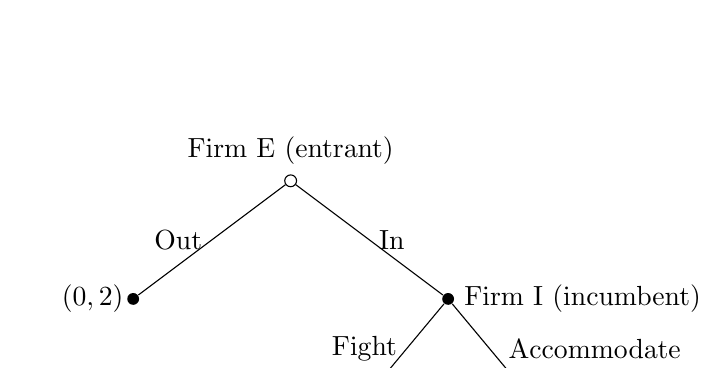
\begin{tikzpicture}[thin,
      level 1/.style={sibling distance=40mm},
      level 2/.style={sibling distance=25mm},
      level 3/.style={sibling distance=15mm},
      every circle node/.style={minimum size=1.5mm,inner sep=0mm}]
      
      \node[circle,draw,label=above:Firm E (entrant)] (root) {}
        child { node [circle,fill,label=above:$$] {}
          node[left] {$(0,2)$}
          edge from parent
            node[left] {Out~}}
        child { node [circle,fill,label=right:Firm I (incumbent)] {}
          child { 
            node {$($-$3,$-$1)$}
              edge from parent
                node[left] {Fight~}}
          child { 
            node {$(2,1)$}
              edge from parent
                node[right] {~Accommodate}}
           edge from parent
             node[right] {In}};
    \end{tikzpicture}
  \end{figure}
  
  	Predation Game in normal form representation:
			\begin{figure}[h!] \centering
  				\begin{game}{2}{2}[Player $1$][Player $2$]
   	    			   	 	& Fight & Accom.    \\
   	 				Out   & $0, 2$ & $0, 2$ \\
   	 				In   & $-3, -1$ & $2, 1$ \\
   	   			\end{game}
			\end{figure} $$ \Rightarrow \text{ two Nash-Equilibria in the normal form game: } (\text{Out, Fight if 'In'}), (\text{In, Accommodate if 'In'}) $$
	But: Is the strategy Fight if ’In’ credible?
\end{example}

\begin{proposition}[Principle of sequential rationality]
	A strategy should specify optimal actions at every point in the game tree given the opponents’ strategies.
\end{proposition}

\begin{proposition}[Backward induction]
	Backward induction is an iterative procedure to identify Nash equilibria that satisfy the principle of sequential rationality in dynamic games:
	\begin{itemize}
		\item Determine the optimal actions at the final decision nodes in the tree.
		\item Derive the reduced extensive form game by deleting the part of the game following these decision nodes and replacing them by the payoffs that result from the optimal play.
		\item Proceed to the next-to-last decision nodes and solve for the optimal actions to be taken there by players who correctly anticipate the actions that will follow at the final nodes.
		\item Continue in this way backwards through the game tree.
	\end{itemize}
\end{proposition}

\begin{example}[Predation Game] ~\\
  \begin{figure}[h!]
 	\centering
    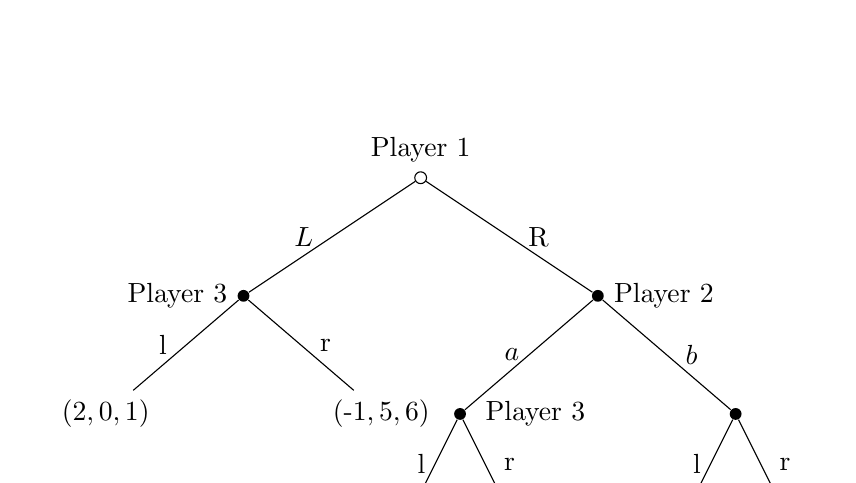
\begin{tikzpicture}[thin,
      level 1/.style={sibling distance=45mm},
      level 2/.style={sibling distance=35mm},
      level 3/.style={sibling distance=15mm},
      every circle node/.style={minimum size=1.5mm,inner sep=0mm}]
      
      \node[circle,draw,label=above:Player 1] (root) {}
        child { node [circle,fill,label=left:Player 3] {}
          child { 
            node {$(2,0,1)$}
              edge from parent
                node[left] {l~~}}
          child { 
            node {$($-$1,5,6)$}
              edge from parent
                node[right] {~r}}
          edge from parent
            node[left] {$L$~~}}
        child { node [circle,fill,label=right:Player 2] {}
          child { node [circle,fill,label=right:~Player 3] {}
          	child { 
              node {$(3,1,2)$}
              	edge from parent
                node[left] {l~}}
            child { 
              node {$(5,4,4)$}
                edge from parent
                node[right] {~r}}
            edge from parent
              node[left] {$a$~}}
          child { node [circle,fill,label=right:$$] {}
          	child { 
              node {$(0,$-$1,7)$}
              	edge from parent
                node[left] {l~}}
            child { 
              node {$($-$2,2,0)$}
                edge from parent
                node[right] {~r}}
            edge from parent
              node[right] {~$b$}}
           edge from parent
             node[right] {~R}};
    \end{tikzpicture}
  \end{figure} $$ \Rightarrow \text{ Equilibrium via backward induction: } (R,a,rrl), \text{ other NEs: e.g. } (L,b,rlr) $$
\end{example}

\begin{theorem}[Zermelo’s Theorem]
Every finite game of perfect information $\Gamma_E$ has a pure strategy Nash equilibrium that can be derived through backward induction. Moreover, if no player has the same payoffs at any two terminal nodes, then there is a unique Nash equilibrium that can be derived in this manner.
\end{theorem}

\begin{example}[Predation Game Version B (Selten, 1865)] ~\\
  \begin{figure}[h!]
 	\centering
    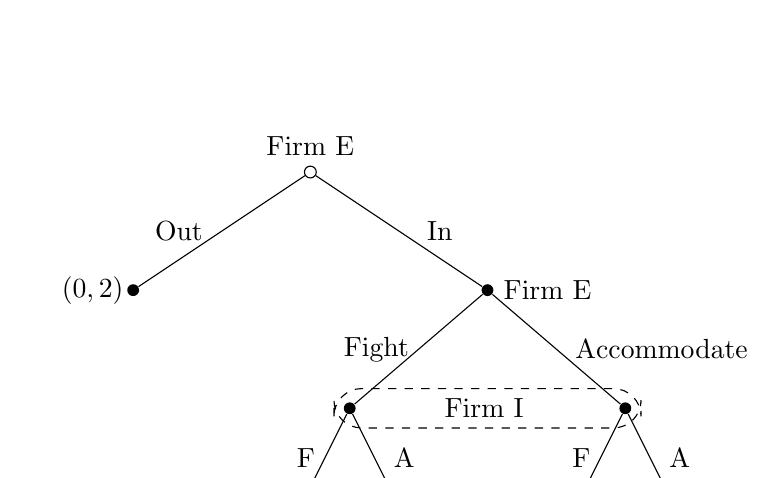
\begin{tikzpicture}[thin,
      level 1/.style={sibling distance=45mm},
      level 2/.style={sibling distance=35mm},
      level 3/.style={sibling distance=15mm},
      every circle node/.style={minimum size=1.5mm,inner sep=0mm}]
      
      \node[circle,draw,label=above:Firm E] (root) {}
        child { node [circle,fill,label=left:] {}
          node[left] {$(0,2)$}
          edge from parent
            node[left] {Out~~}}
        child { node [circle,fill,label=right:Firm E] {}
          child { node(1) [circle,fill,label=right:\hspace{1cm}Firm I] {}
          	child { 
              node {$($-$3,$-$1)$}
              	edge from parent
                node[left] {F~}}
            child { 
              node {$(1,$-$2)$}
                edge from parent
                node[right] {~A}}
            edge from parent
              node[left] {Fight~}}
          child { node(3) [circle,fill,label=right:$$] {}
          	child { 
              node {$($-$2,$-$1)$}
              	edge from parent
                node[left] {F~}}
            child { 
              node {$(3,1)$}
                edge from parent
                node[right] {~A}}
            edge from parent
              node[right] {~Accommodate}}
           edge from parent
             node[right] {~~In}};
            \draw[dashed,rounded corners=10]($(1) + (-.2,.25)$)rectangle($(3) +(.2,-.25)$);
    \end{tikzpicture}
  \end{figure} $$ \Rightarrow \text{ Equilibrium via backward induction: } (R,a,rrl), \text{ other NEs: e.g. } (L,b,rlr) $$ ~\\
	Normal form representation:
			\begin{figure}[h!] \centering
  				\begin{game}{4}{2}[Firm E][Firm I]
   	    			   	 	& A & F    \\
   	 				Out, A if In  & $0, 2$ & \underline{$0, 2$} \\
   	 				Out, F if In  & $0, 2$ & \underline{$0, 2$} \\
   	 				In, A if In  & \underline{$3, 1$} & -$2$, -$1$ \\
   	 				In, F if In  & $1$, -$2$ & -$3$, -$1$ 
   	   			\end{game}
			\end{figure}	
	$$\Rightarrow \text{ Three NEs: } [(\text{Out, A if In}), F],  [(\text{Out, F if In}), F], ~ [(\text{In, A if In}), A] $$

	\textbf{But:} Principle of sequential rationality: A strategy should specify optimal actions at every point in the game tree given the opponents’ strategies.
\end{example}

\begin{definition}[Subgame]
	A subgame of an extensive form game $\Gamma_E$ is a subset of the game having the following properties:
	\begin{enumerate}
		\item It begins with an information set containing a single decision node, contains all the decision nodes that are successors of this node, and contains only these nodes.
		\item If decision node x is in the subgame, then every $x' \in H(x)$ is also, where $H(x)$ is the information set that contains decision node $x$.
	\end{enumerate}
\end{definition} 

\begin{definition}[Subgame Perfect Nash Equilibrium]
	A profile of strategies $\sigma = (\sigma_1, \dotsc, \sigma_l)$ in an $l$-player extensive form game $\Gamma_E$ is a subgame perfect Nash equilibrium (SPNE) if it induces a Nash equilibrium in every subgame of $\Gamma_E$.	
\end{definition}

\begin{proposition}
	Consider an extensive form game $\Gamma_E$ and some subgame $G$ of $\Gamma_E$. Suppose that strategy profile $\gamma^G$ is a SPNE in subgame $G$, and let $\Gamma_E$ be the reduced game formed by replacing subgame $G$ by a terminal node with payoffs equal to those arising from play of $\sigma^G$. Then:
	\begin{enumerate}
		\item In any SPNE $\sigma$ of $\sigma_E$ in which $\sigma^G$ is the play in subgame $G$, players’ moves at information sets outside subgame $G$ must constitute a SPNE of reduced game $\Gamma_E'$.
		\item If $\sigma'$ is a SPNE of $\Gamma_E'$, then the strategy profile $\sigma$ specifies the moves in $\sigma^G$ information sets in subgame $G$ and that specifies the moves in $\sigma'$ at information sets not in $G$ is a SPNE of $\Gamma_E$.
	\end{enumerate}
\end{proposition}

\begin{example}[Niche Choice Game] ~\\
  \begin{figure}[h!]
 	\centering
    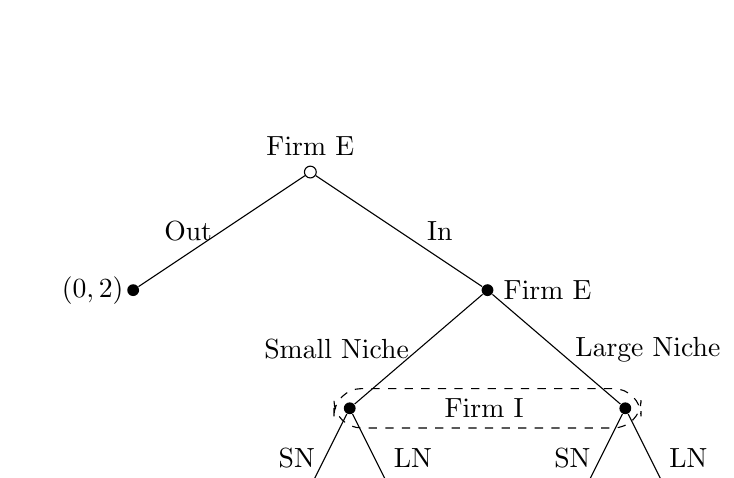
\begin{tikzpicture}[thin,
      level 1/.style={sibling distance=45mm},
      level 2/.style={sibling distance=35mm},
      level 3/.style={sibling distance=15mm},
      every circle node/.style={minimum size=1.5mm,inner sep=0mm}]
      
      \node[circle,draw,label=above:Firm E] (root) {}
        child { node [circle,fill,label=left:] {}
          node[left] {$(0,2)$}
          edge from parent
            node[left] {Out~}}
        child { node [circle,fill,label=right:Firm E] {}
          child { node(1) [circle,fill,label=right:\hspace{1cm}Firm I] {}
          	child { 
              node {$($-$6,$-$6)$}
              	edge from parent
                node[left] {SN~}}
            child { 
              node {$($-$1,1)$}
                edge from parent
                node[right] {~LN}}
            edge from parent
              node[left] {Small Niche~}}
          child { node(3) [circle,fill,label=right:$$] {}
          	child { 
              node {$(1,$-$1)$}
              	edge from parent
                node[left] {SN~}}
            child { 
              node {$($-$3,$-$3)$}
                edge from parent
                node[right] {~LN}}
            edge from parent
              node[right] {~Large Niche}}
           edge from parent
             node[right] {~~In}};
            \draw[dashed,rounded corners=10]($(1) + (-.2,.25)$)rectangle($(3) +(.2,-.25)$);
    \end{tikzpicture}
  \end{figure} 
  
  Post-entry subgame:
			\begin{figure}[h!] \centering
  				\begin{game}{2}{2}[Firm E][Firm I]
   	    			   	 	& SN & LN    \\
   	 				SN  & -$6$, -$6$ & -$1$, $1$ \\
   	 				LN  & $1$, -$1$  & -$3$, -$3$
   	   			\end{game}
			\end{figure}	
  $\Rightarrow$ Two NEs in subgame: $(SN,LN)$, $(LN,SN)$ ~\\

  Normal form representation of the whole game: 
			\begin{figure}[h!] \centering
  				\begin{game}{4}{2}[Firm E][Firm I]
   	    			   	 	& SN & LN    \\
   	 				Out, SN  & $0$, $2$ & \underline{$0$, $2$} \\
   	 				Out, LN  & $0$, $2$ & \underline{$0$, $2$} \\
   	 				In, SN  &  -$6$, -$6$ & -$1$, $1$ \\
   	 				In, LN  & \underline{$1$, -$1$} & -$3$, -$3$ 
   	   			\end{game}
			\end{figure}	  
  $\Rightarrow$ Two SPNE in pure strategies: [$(Out, SN),LN$], [$(In, LN),SN$]. Note: [$(Out, LN),LN$] is not subgame perfect! ~\\
  
  \underline{Period 1:}
  \begin{itemize}
  	\item Player 1 offers a split: $s^1 \in [0, v]$
  	\item Player 2 can reject and the game continues in period 2, or accept and the split is implemented and the game ends immediately with $u_1 = s^1$, $u_2 = v - s^1$.
  \end{itemize}
  
  \underline{Period 2:}
  \begin{itemize}
  	\item Player 2  offers a split: $s^2 \in [0, v]$
  	\item Player 1 can reject and the game continues in period 3, or accept and the split is implemented and the game ends immediately with $u_1 = \delta \cdot s^2$, $u_2 = \delta \cdot (v - s^2)$.
  \end{itemize}
  and so on $\dotsc$ 

  \textbf{There is a unique SPNE:} ~\\

  Suppose T is odd:
  \begin{description}
  	\item \underline{Period T:} Player 1 makes the offer in period T and player 2 is willing to accept any offer. Payoffs: $(\delta^{T-1} \cdot v, 0)$.
  	\item \underline{Period T-1:} Player 2 makes the offer and player 1 will accept if and only if the payoff for player 1 is at least $\delta^{T-1} \cdot v$. Payoffs: $(\delta^{T-1} \cdot v, \delta^{T-2} \cdot v - \delta^{T-1} \cdot v)$.
  	\item \underline{Period T-2:} Player 1 makes the offer and player 2 will accept if and only if the payoff for player 2 is at least $\delta^{T-2} \cdot v - \delta^{T-1} \cdot v$. Payoffs: $(\delta^{T-3} \cdot v - \delta^{T-2} \cdot v + \delta^{T-1} \cdot v, \delta^{T-2} \cdot v - \delta^{T-1} \cdot v)$.
  	\item $\dotsc$
  \end{description}  
  \begin{itemize}
  	\item  The resulting SPNE for odd T is:
		\begin{description}
			\item $v_1^*(T) = v(1 - \delta + \delta^2 - \dotsc + \delta^{T-1}) = v \left[ (1 - \delta) \left(\frac{1 - \delta^{T-1}}{1 - \delta^2} \right) + \delta^{T-1} \right]$
			\item $v_2^*(T) = v - v_1^*(T)$
		\end{description}
	\item The resulting SPNE for even T is:
		$$ v_1^*(T) = v - \delta v_1^*(T-1), \quad v_2^*(T) = v_1^*(T - 1). $$
  \end{itemize}
  $\Rightarrow$ For large T, this converges to:
 	$$ \lim_{T \rightarrow \infty} v_1^*(T) = \frac{v}{1 + \delta}, \quad \lim_{T \rightarrow \infty} v_2^*(T) = \frac{\delta v}{1 + \delta}$$
\end{example} 

Now consider the bilateral bargaining gam with infinite horizon:

\begin{proposition}[Shaked \& Sutton (1984)]
	The infinite horizon bargaining game has a unique SPNE in which the players reach an agreement in period 1 such that player 1 earns $\frac{v}{1 + \delta}$ and player 2 $\frac{\delta v}{1 + \delta}$.
	
	\begin{proof}
		Let $\overline{v_1}$ be the largest payoff that player 1 gets in any SPNE. Then player 1's payoff in any SPNE cannot be lower than $\underline{v_1} = v - \delta \overline{v_1}$. Also $overline{v_1} \leq v - \delta \underline{v_1}$ because player 2 rejects any offer of less than $\delta \underline{v_1}$. And we have:
		$$ \overline{v_1} \leq v - \delta \underline{v_1} = \underline{v_1} + \delta \overline{v_1} - \delta \underline{v_1} \iff \overline{v_1} (1 - \delta) \leq \underline{v_1} (1 - \delta). $$
		Which implies $\overline{v_1} = \underline{v_1}$, so player 1's SPNE is uniquely determined:
		$$ \Rightarrow v_1^0 = v - \delta v_1^0 = \frac{v}{1 + \delta} \text{ and } v_2^0 = \frac{\delta v}{1 + \delta} $$ 
	\end{proof}
\end{proposition}

% todo 952 Kooperative Spiele
\chapter{Kooperative Spiele} 


Im Kontrast zur nicht-kooperativen Spieltheorie, die sich mit Spielern die individuell Entscheidungen treffen und ihre individuelle Auszahlung ohne Absprache maximieren, beschäftigt, gibt es die kooperative Spieltheorie, mit der wir uns im folgenden beschäftigen. In der kooperativen Spieltheorie können sich die Spieler gemeinsam auf Ergebnis einigen, die dann auch verpflichtend sind. Man braucht dazu Kontrollinstanzen; Wir suchen nach Stabilität und Ergebnissen, die sich in solchen Situationen ergeben.

\subsubsection*{Koalitionsspiele (Spiele in charakteristischer Form)}
\begin{itemize}
	\item Die Modellierung als Koalitionsspiel wird angewendet, wenn bindende Absprachen möglich sind. 
	\item Im Fokus: Was kann eine Gruppe von Spielern (eine \textit{Koalition}) gemeinsam erreichen? 
	\item Es wird dabei nicht betrachtet, wie die Koalition dies erreicht, d.h. wie sie ihre gemeinsamen Aktionen abstimmt. 
	\item Fragen: Wie wird sie dies aufteilen? Wie sollte sie dies aufteilen? Gibt es stabile Aufteilungen? 
	\item \textit{Lösung eines Koalitionsspiels}: (Menge an) Payoffvektoren mit bestimmten Eigenschaften.
\end{itemize}

Wir betrachten nur Koalitionsspiele mit transferierbarem Nutzen, also Spiele bei denen der Wert, den eine Koalition erreichen kann, beliebig unter den Mitgliedern aufgeteilt werden kann.

\begin{definition}[Koalitionsspiel mit transferierbarem Nutzen]
	Ein Koalitionsspiel $(N, v)$ mit tranferierbarem nutzen besteht aus
	\begin{itemize}
		\item einer endlichen Menge $N = \{1, \dotsc, n\}$ an Spielern und
		\item einer charakteristischen Funktion $v \colon \mathcal{P}(N) \rightarrow \mathbb{R}$, die jeder Teilmenge $S$ von $N$ einen (Koalitions-) Wert $v(\mathcal{S})$ zuweist.
	\end{itemize}
	($\mathcal{P}(N)$ ist die Potenzmenge von $N$.)
\end{definition} 

\begin{bemerkung} ~\
  \begin{itemize}
	\item Die charakteristische Funktion wird auch Koalitionsfunktion genannt.
	\item Wir treffen die Annahme, dass Aktionen von Spielern in $N \setminus S$ den Wert $v(S)$ nicht beeinflussen (vgl. \enquote{outside option}).
	\item Wir interpretieren $v(S)$ als den Payoff, den sich die Koalition $S$ aus eigener Kraft sichern kann.
	\item Es gelte $v(\emptyset) = 0$.
	\item Die Spieler in S entscheiden über mögliche Aufteilungen von $v(S)$ auf die Spieler in $S$ (da der Nutzen transferierbar ist).	
  \end{itemize}	
\end{bemerkung}

Stille Annahme: Existenz einer übergeordneten Kontrollinstanz.~\\

Zur Vereinfachung betrachten wir im Folgenden superadditive Spiele: Eine Koalition $S \cup T$ kann immer mindestens das erreichen, was ihre disjunkten Teilkoalitionen $S$ und $T$ getrennt erreichen können.

\begin{definition}[Superadditive Spiele]
	Ein Koalitionsspiel $(N, v)$ ist superadditiv, wenn
	$$ v(S \cup T) \geq v(s) + v(t) $$
	für alle Koalitionen $S$ und $T$ mit $S \cap T = \emptyset$.
\end{definition}
	
Bei der Analyse von Koalitionsspielen spielt der Payoff, den die einzelnen Spieler erhalten, eine Rolle.
\begin{itemize}
	\item Ein Payoffvektor sei bezeichnet mit $x = (x_1, \dotsc, x_n)$.
	\item Der Gesamtpayoff, den die Spieler einer Gruppe $S$ erhalten ist also $\sum_{i \in S} x_i$.
	\item Anmerkung: Hier betrachten wir einen Payoffvektor und berechnen, wie hoch der gemeinsame Payoff der Spieler in $S$ ist. Dies hat nichts mit $v(S)$ zu tun, dem Payoff, den die Koalition $S$ aus eigener Kraft erreichen kann.
\end{itemize} 

\begin{definition}[Zulässiger Payoffvektor]
	In einem superadditiven Spiel ist ein Payoffvektor $x$ zulässig, wenn
	$$ \sum_{i \in N} x_i \leq v(N) $$
\end{definition} ~\\
	
Wir werden zwei Lösungskonzepte kennen lernen:
\begin{itemize}
	\item Ein Mengenkonzept, das eine Menge von Payoffvektoren als Lösung vorschlägt: der Kern.
	\item Ein Wertkonzept, das eine eindeutige Lösung des Spiels vorschlägt: der Shapley-Wert.
\end{itemize}

% todo 1016 Der Kern
\section{Der Kern} 

\begin{itemize}
	\item Der Kern enthält alle \enquote{stabilen} Payoffvektoren.
	\item Idee: Ein Payoffvektor eines Koalitionsspiels ist stabil, wenn es keine Koalition gibt, die aus eigener Kraft für jedes ihrer Mitglieder einen höheren Payoff erzielen könnte.
	\item Bei transferierbarem Nutzen: Ein Payoffvektor ist stabil, wenn es keine Koalition gibt, deren Wert höher ist als die Summe der Payoffs ihrer Mitglieder (im betrachteten Payoffvektor).
	\item Da wir nur superadditive Spiele betrachten, wird immer die große Koalition den Gesamtpayoff der Kernlösung (falls diese existiert) bestimmen.
	\item Der Kern kann aus mehreren Payoffvektoren bestehen, er kann eindeutig sein und er kann leer sein.
\end{itemize}

\begin{definition}[Kern]
	Der Kern eines Koalitionsspiels mit transferierbarem Nutzen $(N, v)$ ist die Menge zulässiger Payoffvektoren $x$, für die gilt
	$$ \sum_{i \in S} x_i \geq v(S) $$
	für alle $S \subseteq N$.
\end{definition}

\textbf{Eigenschaften:}
\begin{itemize}
	\item Das bedeutet, dass keine Koalition einen Payoffvektor im Kern blockieren kann: $\exists! S \subseteq N$, so dass $v(S) > \sum_{i \in S} x_i$.
	\item Payoffvektoren im Kern sind individuell rational: $x_i \geq v(i)$.
	\item Da der Kern eine Menge an Payoffvektoren ist, welche Lösung eines Systems linearer Ungleichungen sind, ist er eine abgeschlossene und konvexe Menge.
\end{itemize}

\begin{unnamedtheorem}[Bedeutung des Kerns] ~\
	\begin{enumerate}
		\item Ein Payoffvektor, der nicht im Kern liegt, ist als Lösung instabil: Mindestens eine Koalition wird der Absprache nicht zustimmen.
		\item Wenn der Kern leer ist, gibt es keine Aufteilung des Gesamtwerts der großen Koalition (in superadditiven Spielen), welcher alle Gruppen zustimmen würden. Damit sind die Voraussetzungen für eine Aufteilung der Payoffs schlecht. Zum Beispiel kann dies bei der Gewinn- oder Kostenaufteilung in Unternehmen oder in Wertschöpfungsketten eine Rolle spielen.
	\end{enumerate} 
\end{unnamedtheorem}
 
\begin{beispiel}[Abstimmungsspiel 1] ~\
	\begin{itemize}
		\item Drei Spieler wollen ein homogenes Gut mit Wert Eins aufteilen. 
		\item Abstimmungsregel: Die Mehrheit muss der vorgeschlagenen Aufteilung zustimmen.
	\end{itemize}
	Welche Aufteilungen liegen im Kern? ~\\
	
	Formalisierung des Abstimmungsspiels (wobei im Folgenden werden Spielermengen vereinfacht ohne Klammer dargestellt)
	\begin{itemize}
		\item Menge der Spieler: $\{1, 2, 3\}$
		\item Charakteristische Funktion: Was kann sich eine Koalition aus eigener Kraft sichern? ~\\
			Wenn die Koalition aus der Mehrheit der Spieler besteht, kann sie die Abstimmung in ihrem Sinne entscheiden. Wenn sie aus der Minderheit besteht, kann sie gegen den Willen der anderen nichts erreichen.
				\begin{itemize}
					\item $v(S) = 1$ für alle $S$ mit $|S| \geq 2$
					\item $v(S) = 0$ für alle $S$ mit $|S| < 2$
				\end{itemize}
	\end{itemize}
	Der Kern ist die Menge der Lösungen des folgenden Systems linearer Ungleichungen:
	\begin{align*}
		x_1 + x_2 + x_3 & = v(123) = 1 \\
		x_1 + x_2 & \geq v(12) = 1 \\
		x_1 + x_3 & \geq v(13) = 1 \\
		x_2 + x_3 & \geq v(23) = 1 \\
		x_1 & \geq v(1) = 0 \\
		x_2 & \geq v(2) = 0 \\
		x_3 & \geq v(3) = 0 		
	\end{align*}
	Der Kern ist leer:
	$$ x_1 + x_2 + x_3 = 1 \text{ und } x_1 + x_2 \geq 1 \text{ und } x_3 \geq 0 \Rightarrow x_3 = 0 $$
	$$ x_1 + x_2 + x_3 = 1 \text{ und } x_1 + x_3 \geq 1 \text{ und } x_3 \geq 0 \Rightarrow x_2 = 0 $$
	$\Rightarrow x_2 + x_3 = 0$, ein Widerspruch zu $x_2 + x_3 \geq 1$.
\end{beispiel}
 
\begin{beispiel}[Abstimmungsspiel 2] ~\
	\begin{itemize}
		\item Drei Spieler wollen ein homogenes Gut mit Wert Eins aufteilen. 
		\item Abstimmungsregel: Alle müssen der vorgeschlagenen Aufteilung zustimmen.
	\end{itemize}
	Welche Aufteilungen liegen im Kern?
	\begin{align*}
		x_1 + x_2 + x_3 & = v(123) = 1 \\
		x_1 + x_2 & \geq v(12) = 0 \\
		x_1 + x_3 & \geq v(13) = 0 \\
		x_2 + x_3 & \geq v(23) = 0 \\
		x_1 & \geq v(1) = 0 \\
		x_2 & \geq v(2) = 0 \\
		x_3 & \geq v(3) = 0 		
	\end{align*}
	Kern: alle $(x_1, x_2, x_3)$ mit $x_1 + x_2 + x_3 = 1$ und $x_1 \geq 0$, $x_2 \geq 0$, $x_3 \geq 0$.
\end{beispiel} 
 
\begin{beispiel}[Abstimmungsspiel 2] ~\
	\begin{itemize}
		\item Drei Spieler wollen ein homogenes Gut mit Wert Eins aufteilen. 
		\item Abstimmungsregel: Mindestens 50\% Stimmgewicht muss zustimmen.
		\item Stimmgewicht der drei Spieler: 60\%, 20\%, 20\%
	\end{itemize}
	Welche Aufteilungen liegen im Kern?
	\begin{align*}
		x_1 + x_2 + x_3 & = v(123) = 1 \\
		x_1 + x_2 & \geq v(12) = 1 \\
		x_1 + x_3 & \geq v(13) = 1 \\
		x_2 + x_3 & \geq v(23) = 0 \\
		x_1 & \geq v(1) = 1 \\
		x_2 & \geq v(2) = 0 \\
		x_3 & \geq v(3) = 0 		
	\end{align*}
	Der Kern ist eindeutig: $(1, 0, 0)$.
\end{beispiel} 
  
% todo 1117 Der Shapley-Wert
\section{Der Shapley-Wert}

\begin{itemize}
	\item Im Gegensatz zum Kern ist der Shapley-Wert ein Wertkonzept, d.h. eine Lösungsfunktion, die genau einen Payoffvektor als Lösung auswählt.
	\item Er schlägt eine Aufteilung des gemeinschaftlich erreichten Werts vor, die in gewissem Sinne \enquote{fair} ist. Er kann in vielen Spielen auch als Machtindex interpretiert werden.
	\item Die Idee hinter dem Shapley-Wert ist, dass jeder Spieler den Durchschnitt seiner marginalen Beiträge zum Wert aller möglichen Koalitionen bekommt.
	\item Der Shapley-Wert kann auch axiomatisch begründet werden.
\end{itemize}

\begin{definition}[Shapely-Wert]
	Der Shapley-Wert $\phi(N, v) = \left( \phi_1(N,v), \dotsc, \phi_n(N,v) \right)$ im Koalitionsspiel $(N, v)$ ist gegeben durch
	$$ \phi_i(N,v) = \frac{1}{n!} \sum_{\pi \in \pi_N} \left( v\left(S_i(\pi) \cup \{ i \} \right) - v\left(S_i(\pi)\right) \right) $$
	für alle $i \in N$.
\end{definition}

\begin{itemize}
	\item $\pi_N$ ist die Menge aller möglichen Spielerreihenfolgen. Es gibt $n!$ Reihenfolgen.
	\item $S_i(\pi)$: Menge an Spielern, die in der Reihenfolge $\pi$ vor $i$ kommen.
	\item Alternative Darstellung:
		$$ \phi_i(N,v) = \sum_{S \subseteq N \setminus \{ i \}}\frac{\left( n - |S| - 1 \right)!\left(|S|\right)!}{n!} \left( v\left( S \cup \{i\} \right) v(S) \right). $$
\end{itemize}

\textbf{Intuition} ~\\
Wenn die Koalition durch sequentielles Eintreten der Spieler gebildet wird und jeder Spieler seinen Beitrag $v(S \cup \{ i \}) - v(S)$ zur bisherigen Koalition $S$ als faire Entschädigung verlangt, dann entspricht $\phi_i(N, V)$ diesem Wert, wenn man den Durchschnitt über alle möglichen Reihenfolgen betrachtet, gemä{\ss} derer die Koalition $N$ sich bilden kann. ~\\

Es kann gezeigt werden, dass der Shapley-Wert $\phi(N, v)$ der einzigen Lösung $\varphi(N, v)$ entspricht, die folgenden vier Axiome für alle $(N, v)$ erfüllt.

\begin{unnamedtheorem}[Axiomatische Begründung] ~\
	\begin{enumerate}
		\item[A1] Effizienz: $\sum_{i \in N} \varphi_i(N,v) = v(N)$ ~\\
			\textit{Dieses Axion verlangt, dass keine möglichen Nutzen verloren gehen. Alles was die große Koalition erreicht, wird aufgeteilt.}
		\item[A2] Symmetrie: Wenn für zwei Spieler $i$ und $j$ gilt, dass
			$$ v\left( S \cup \{i\} \right) - v(S) = v\left( S \cup \{j\} \right) - v(S) $$
			für alle $S$ in denen $i$ und $j$ nicht enthalten sind, dann gilt $\varphi_i(N,v) = \varphi_j(N,v)$. ~\\
			\textit{Dieses Axiom verlangt, dass eine Lösung nicht von der Bezeichnung der Spieler abhängt. Wenn Spieler austauschbar sind (da sie zu jeder Koalition dasselbe beitragen) dann soll auch ihr Wert der selbe sein.}
		\item[A3] Null-Spieler: Wenn für einen Spieler $i$ gilt, dass
			$$ v\left( S \cup \{i\} \right) - v(S) = 0 $$
			für alle $S$, dann gilt $\varphi_i(N, v) = 0$. ~\\
			\textit{Wenn ein Spieler zu keiner Koalition etwas beiträgt, soll er auch nichts erhalten.}	
		\item[A4] Additivität: Ein Wert $\varphi$ erfüllt Additivität, wenn für jedes Paar von Spielen $(v, N)$ und $(w, N)$ gilt
			$$ \varphi_i(v + w, N) = \varphi_i(v, N) + \varphi_i(w, N) $$
			für alle $i \in N$, wobei $(v + w, N)$ definiert sei durch $(v + w)(S) = v(S) + w(S)$ für alle $S \subseteq N$.
			\textit{Wenn die Koalitionswerte zweier Spiele jeweils addiert ein anderes Spiel ergeben, dann soll auch der Wert jedes Spielers die Summe seiner Werte in den beiden Spielen sein.}
	\end{enumerate}
\end{unnamedtheorem}

\begin{satz}
	Der Shapley-Wert $\phi(N, v)$ ist der einzige wert, der A1-A4 erfüllt.
\end{satz}

Man kann den Shapley-Wert auch über andere Axiomensysteme charakterisieren.
~\newpage
\begin{beispiel}[Abstimmungsspiel 1] ~\
	\begin{itemize}
		\item Drei Spieler wollen ein homogenes Gut mit Wert Eins aufteilen. 
		\item Abstimmungsregel: Die Mehrheit muss der vorgeschlagenen Aufteilung zustimmen.
	\end{itemize}
	Welche Aufteilungen liegen im Kern? Welche Aufteilung schlägt der Shapley-Wert als Lösung vor?
	\begin{align*}
		x_1 + x_2 + x_3 & = v(123) = 1 \\
		x_1 + x_2 & \geq v(12) = 1 \\
		x_1 + x_3 & \geq v(13) = 1 \\
		x_2 + x_3 & \geq v(23) = 1 \\
		x_1 & \geq v(1) = 0 \\
		x_2 & \geq v(2) = 0 \\
		x_3 & \geq v(3) = 0 		
	\end{align*}
	Der Kern ist leer: 
	\begin{itemize}
		\item $x_1 + x_2 + x_3 = 1$ und $x_1 + x_2 \geq 1 \Rightarrow x_3 = 0$
		\item $x_1 + x_2 + x_3 = 1$ und $x_1 + x_e \geq 1 \Rightarrow x_w = 0$
		\item $\Rightarrow x_2 + x_3 = 0$, ein Widerspruch zu $x_2 + x_3 \geq 1$
	\end{itemize} ~\newpage
	Shapley-Wert: ~\\
	  \begin{figure*}[h!] \centering
		\begin{tabular}{cc}
  			\hline
  				Reihenfolge & marginaler Beitrag Spieler 1/2/3 \\
  			\hline
  				123 & 0/1/0 \\
  				132 & 0/0/1 \\
  				213 & 1/0/0 \\
  				231 & 0/0/1 \\
  				312 & 1/0/0 \\
  				321 & 0/1/0 \\
  			\hline
		\end{tabular}
	\end{figure*}
	\begin{itemize}
		\item Shapley-Wert: $\left( \frac{1}{3}, \frac{1}{3}, \frac{1}{3} \right)$ (z.B. ist der durchschnittliche marginale Beitrag von Spieler 1 $\phi_1(N, v) = (0+0+1+0+1+0)/6 = 1/3$.)
	\end{itemize}
	Der Shapley-Wert ist $\left( \frac{1}{3}, \frac{1}{3}, \frac{1}{3} \right)$ und der Kern ist leer.
\end{beispiel}

\begin{beispiel}[Abstimmungsspiel 2] ~\
	\begin{itemize}
		\item Drei Spieler wollen ein homogenes Gut mit Wert Eins aufteilen. 
		\item Abstimmungsregel: alle müssen der vorgeschlagenen Aufteilung zustimmen.
	\end{itemize}
	Welche Aufteilungen liegen im Kern und welche schlägt der Shapley-Wert als Lösung vor?
	\begin{align*}
		x_1 + x_2 + x_3 & = v(123) = 1 \\
		x_1 + x_2 & \geq v(12) = 0 \\
		x_1 + x_3 & \geq v(13) = 0 \\
		x_2 + x_3 & \geq v(23) = 0 \\
		x_1 & \geq v(1) = 0 \\
		x_2 & \geq v(2) = 0 \\
		x_3 & \geq v(3) = 0 		
	\end{align*}
	Kern: Alle $(x_1, x_2, x_3)$ mit $x_1 + x_2 + x_3 = 1$ und $x_1 \geq 0$, $x_2 \geq 0$, $x_3 \geq 0$. Shapley-Wert: ~\\
	  \begin{figure*}[h!] \centering
		\begin{tabular}{cc}
  			\hline
  				Reihenfolge & marginaler Beitrag Spieler 1/2/3 \\
  			\hline
  				123 & 0/0/1 \\
  				132 & 0/1/0 \\
  				213 & 0/0/1 \\
  				231 & 1/0/0 \\
  				312 & 0/1/0 \\
  				321 & 1/0/0 \\
  			\hline
		\end{tabular}
	\end{figure*}
	\begin{itemize}
		\item Shapley-Wert: $\left( \frac{1}{3}, \frac{1}{3}, \frac{1}{3} \right)$ (z.B. ist der durchschnittliche marginale Beitrag von Spieler 1 $\phi_1(N, v) = (0+0+0+1+0+1)/6 = 1/3$.)
	\end{itemize}
	Der Shapley-Wert schlägt eine gleichmäßige Aufteilung vor, die im Kern liegt.
\end{beispiel}

\begin{beispiel}[Abstimmungsspiel 3] ~\
	\begin{itemize}
		\item Drei Spieler wollen ein homogenes Gut mit Wert Eins aufteilen. 
		\item Abstimmungsregel: Mindestens 50\% Stimmgewicht muss zustimmen.
		\item Stimmengewicht der drei Spieler: 60\%, 20\%, 20\%
	\end{itemize}
	Welche Aufteilungen liegen im Kern? Welche Aufteilung schlägt der Shapley-Wert als Lösung vor?
	\begin{align*}
		x_1 + x_2 + x_3 & = v(123) = 1 \\
		x_1 + x_2 & \geq v(12) = 1 \\
		x_1 + x_3 & \geq v(13) = 1 \\
		x_2 + x_3 & \geq v(23) = 0 \\
		x_1 & \geq v(1) = 1 \\
		x_2 & \geq v(2) = 0 \\
		x_3 & \geq v(3) = 0 		
	\end{align*}
	Der Kern ist eindeutig: (1, 0, 0). ~\newpage
	Shapley-Wert: ~\\
	  \begin{figure*}[h!] \centering
		\begin{tabular}{cc}
  			\hline
  				Reihenfolge & marginaler Beitrag Spieler 1/2/3 \\
  			\hline
  				123 & 1/0/0 \\
  				132 & 1/0/0 \\
  				213 & 1/0/0 \\
  				231 & 1/0/0 \\
  				312 & 1/0/0 \\
  				321 & 1/0/0 \\
  			\hline
		\end{tabular}
	\end{figure*}
	\begin{itemize}
		\item Shapley-Wert: $\left( 1, 0, 0 \right)$ (z.B. ist der durchschnittliche marginale Beitrag von Spieler 1 $\phi_1(N, v) = (1+1+1+1+1+1)/6 = 1$.)
	\end{itemize}
	Der Shapley-Wert stimmt mit der eindeutigen Kern-Lösung überein.
\end{beispiel}

\begin{beispiel}[Abstimmungsspiel 4] ~\
	\begin{itemize}
		\item Drei Spieler wollen ein homogenes Gut mit Wert Eins aufteilen. 
		\item Abstimmungsregel: Mindestens 75\% Stimmgewicht muss zustimmen.
		\item Stimmengewicht der drei Spieler: 60\%, 20\%, 20\%
	\end{itemize}
	Welche Aufteilungen liegen im Kern? Welche Aufteilung schlägt der Shapley-Wert als Lösung vor?
	\begin{align*}
		x_1 + x_2 + x_3 & = v(123) = 1 \\
		x_1 + x_2 & \geq v(12) = 1 \\
		x_1 + x_3 & \geq v(13) = 1 \\
		x_2 + x_3 & \geq v(23) = 0 \\
		x_1 & \geq v(1) = 0 \\
		x_2 & \geq v(2) = 0 \\
		x_3 & \geq v(3) = 0 		
	\end{align*}
	Der Kern ist eindeutig: (1, 0, 0)
	\begin{itemize}
		\item $x_1 + x_2 + x_3 = 1$ und $x_1 + x_2 \geq 1 \Rightarrow x_3 = 0, x_1 + x_2 = 1$
		\item $x_1 + x_2 + x_3 = 1$ und $x_1 + x_3 \geq 1 \Rightarrow x_2 = 0$
		\item $x_1 + x_2 = 1$ und $x_2 = 0 \Rightarrow x_1 = 1$
	\end{itemize} ~\newpage
	Shapley-Wert: ~\\
	  \begin{figure*}[h!] \centering
		\begin{tabular}{cc}
  			\hline
  				Reihenfolge & marginaler Beitrag Spieler 1/2/3 \\
  			\hline
  				123 & 0/1/0 \\
  				132 & 0/0/1 \\
  				213 & 1/0/0 \\
  				231 & 1/0/0 \\
  				312 & 1/0/0 \\
  				321 & 1/0/0 \\
  			\hline
		\end{tabular}
	\end{figure*}
	\begin{itemize}
		\item Shapley-Wert: $\left( \frac{2}{3}, \frac{1}{6}, \frac{1}{6} \right)$ (z.B. der durchschnittliche marginale Beitrag von Spieler 1: $\phi_1(N, v) = (0+0+1+1+1+1)/6 = 2/3$.)
	\end{itemize}
	Der Shapley-Wert schlägt die Aufteilung $\left( \frac{2}{3}, \frac{1}{6}, \frac{1}{6} \right)$ vor und die eindeutige Kern-Lösung ist $(1, 0, 0)$.
\end{beispiel}

% todo 1329 Einfache Spiele
\section{Einfache Spiele} 

\begin{definition}[Einfaches Spiel]
	Ein Koalitionsspiel $(N, v)$ hei{\ss}t einfach, wenn für jede Koalition $S \subseteq N$ entweder $v(S) = 0$ und $v(S) = 1$ gilt.
\end{definition}

\begin{itemize}
	\item Eine Koalition $S$ für die $v(S) = 1$ gilt hei{\ss}t Gewinnerkoalition.
	\item Ein Spieler, der in jeder Gewinnerkoalition des Spiels ist, hei{\ss}t Veto-Spieler.
\end{itemize} ~\newpage

\begin{satz} ~\
	\begin{itemize}
		\item Wenn es in einem einfachen Spiel keinen Veto-Spieler gibt, ist der Kern leer.
		\item Wenn es in einem einfachen Spiel (einen oder mehrere) Veto-Spieler gibt, besteht der Kern aus allen nicht-negativen zulässigen Payoffvektoren, in denen die anderen (Nicht-Veto-)Spieler Null erhalten.
	\end{itemize}
\end{satz}

\section{Konvexe Spiele} 

Gibt es eine Charakterisierung von Spielen, für die der Shapley-Wert im Kern liegt?

\begin{definition}[Konvexes Spiel]
	Ein Spiel heißt konvex, wenn für jeden Spieler $i$ der marginale Beitrag von $i$ grö{\ss}er ist wenn die Koalition wächst; genauer, wenn für alle $S \subset T$ und $i \in N \setminus T$ gilt, dass
	$$ v( S \cup \{i\}) - v(S) \leq v( T \cup \{ i \}) - v(T). $$
\end{definition}

\begin{satz}
	Der Shapley-Wert eines konvexen Spiels liegt im Kern.
\end{satz}
Aus diesem Satz folgt direkt, dass der Kern eines konvexen Spiels nicht leer ist.

% todo 1362 Evolutionäre Spieltheorie
\chapter{Evolutionäre Spieltheorie}

  
\section{Spiele in Normalform}
Für symmetrische Spiele:
$$ A = \left( a_{ij} \right) \quad i = 1, \dotsc, m_{i}, ~ j = 1, \dotsc, m_{j} $$
d.h.
\begin{figure*}[h!] \centering
 \begin{tabular}{l|ccc}
   ~                & $\sigma_{21}$ & $\dotsc$  & $\sigma_{2 m_{2}} $\\
  \hline
  $\sigma_{11}$     &  $a_{11}$     & $\dotsc$  & $a_{1m_{2}}$ \\
  $\vdots$          & $\vdots$      & ~         & $\vdots$ \\
  $\sigma_{1m_{1}}$ & $a_{m_{1} 1}$ & $\dotsc $ & $a_{m_{1} m_{2}}$
 \end{tabular}	
\end{figure*}

\begin{description}
	\item $N$: Spielermenge $|N| = n$
	\item $\Sigma_{i}$: Menge der reinen Strategien von $i \in N$, $\left| \Sigma_{i} \right| = m_{i}$, $\sigma_{i} \in \mathcal{E}_{i}$.
	\item $S_{i}$: Menge der gemischten Strategien von $i \in N$
		\begin{description}
			\item $S_{i} = \left\{ s_i \in \mathbb{R}^m_i : \sum_{j=1}^{m_i} s_{ij} = 1, s_{ij} \geq 0 \text{ für alle} j = 1, \dotsc, m_i \right\}$.
			\item $s_{ij} = \mathds{P}(\sigma_{ij})$.
		\end{description}
\end{description}
  
\begin{definition}[Trägermenge] Wir definieren die Trägermenge für jeden Spieler $i \in N$:
	$$ C(S_{i}) = \left\{ \sigma_{ij} \in \Sigma_{i} : s_{ij} > 0 \right\}, $$
	als die Menge der Strategien die mit positiver Wahrscheinlichkeit gespielt werden.
\end{definition}  

\begin{definition}[Beste-Antwort-Menge] Sei
	$$ B_{i}(s_{-i}) = \left\{ \sigma_{j} \in \Sigma_{i} : H(\sigma_{ij}, s_{-i}) = \max_{\sigma_{ik \in \Sigma_{i}}} H(\sigma_{ik}, s_{-i}) \right\} $$ 
	$H$ bezeichne pay-off-Funktion ~\\
	$$ \hat{H}(s_{-i}) \coloneqq \max_{\sigma_{il} \in \Sigma_{i}} H(\sigma_{ik}, s_{-i}) $$
\end{definition}
  
  
\begin{beispiel*}
	$\sigma_{ij} \in B_{i}(S_{-i})$ und $\sigma_{ik} \in B(S_{-i}) \Rightarrow$ alle $s_{i} \in S_{i}$ mit
	$$ C(S_{i}) = \{ \sigma_{ij}, \sigma_{ik} \} $$	
	sind auch beste Antwort, denn
	$$ s_{ij} H(\sigma_{j}, s_{-i}) + s_{ik} H(\sigma_{ik}, s_{-i}) = (s_{ij} + s_{ik}) \hat{H}(s_{-i}) = \hat{H}(s_{-i}). $$
\end{beispiel*}

Sei $s^{*} = \left( s_{1}^{*}, \dotsc, s_{n}^{*} \right)$ ein Nash-Gleichgewicht. Mit $s_{i}^{*} = (s_{i1}^{*}, \dotsc s_{im_{i}}^{*})$ gilt
$$ C(s_{i}^{*}) \subseteq B_{i}(s_{-i}^{*}) $$
 \textit{Hinreichend? Ja! Proposition Slide 36 (AGT Teil 1)}.


\begin{unnamedtheorem}[Grundannahmen der evolutionären Spieltheorie]
	\begin{enumerate}
		\item große Population
		\item Population ist monomorph
		\item random matching
		\item Wettstreit (Spiel) ist statisch und symmetrisch
			$$ \Rightarrow \text{ symmetrisches Spiel in Normalform mit zwei Spielern}. $$
		\item Auszahlung entspricht der \enquote{biologischen Fitness} ($\phi$ Anzahl Nachkommen)
		\item Reproduktion ist asexuell und die von den Eltern gewählt Strategie wird unverändert an die Nachkommen vererbt (nur Selektion, keine Mutation).
	\end{enumerate}
\end{unnamedtheorem} 
 

\begin{unnamedtheorem}[Symmetrisches 2-Personenspiel in Normalform]
	Spieler müssen nicht unterschieden werden $\Rightarrow$ Strategieraum:
	$$ S = \{ s\in \R^{m} : \sum_{i=1}^{m} s_{i} = 1, s_{i} \geq 0, i = 1, \dotsc, m \} $$
\end{unnamedtheorem}
  
 
\begin{definition}[Evolutionär stabile Strategie, ESS]
	Eine Strategie $p \in S$ hei{\ss}t evolutionär stabil, wenn
	\begin{enumerate}
		\item $H(p,p) \geq H(q, p)$ für alle $q \in S$ (Gleichgewichtsbedingung)
		\item Für alle $q \in S \setminus \{ p \}$ mit $H(q, p) = H(p, p)$ gilt: $H(p, q) > H(q, q)$ (Stabilitätsbedingung)
	\end{enumerate}
\end{definition}  


\begin{unnamedtheorem}[Eigenschaften von evolutionär stabilen Strategien] ~\
	\begin{itemize}
		\item Ist $p \in S$ eine evolutionär stabile Strategie, dann bildet $(p, p)$ ein symmetrisches Nash-Gleichgewicht
		\item Jede $2 \times 2$-Matrix $A = \begin{pmatrix}
			a_{11} & a_{12} \\ a_{21} & a_{22}
		\end{pmatrix}$ mit $H(p,p) = p'Ap$ sodass $a_{11} \neq a_{21}$ und / oder $a_{12} = a_{22}$, besitzt eine ESS
		Ist $(p,p)$ ein striktes NGG, dann ist $p$ eine ESS. Im strikten NGG $(p, p)$ gilt $C(p) = B(p)$. Ein striktes NGG ist immer ein Gleichgewicht in reinen Strategien. Beispiel:
   \begin{game}{2}{2}[~][]
   	    &  ~      &  ~     \\
   	 ~  &    $3, 3$      & $2, 0$  \\
   	  	&  $0, 2$ & $4, 4$\\
   \end{game}
	\item Im Normalformspielen mit $m \times m$-Matrizen $a$ mit $m \geq 3$ existieren entweder endlich viele ESS keine.
	\end{itemize}
\end{unnamedtheorem}
  
\begin{unnamedtheorem}[Allgemein gilt]
	Ist $p$ ESS $\Rightarrow \neg \exists \sigma \in C(p)$ mit $\sigma \in C(S^{*})$ für $s^{*} \neq q$ ist Nash-Gleichgewicht
\end{unnamedtheorem} 

$\Rightarrow \#$ ESS $\leq \left| \Sigma \right|$ - Gleichheit nur, fall es kein ESS in gemischten Strategien gibt.  
    
% todo 1464 Übungen
\newpage \phantomsection \appendix 
\chapter{Übungen}


\section{Exercises to noncooperative Games}

\subsection*{Advanced Game Theory - 1. Exercise}

\subsubsection*{Exercise 1.1}

In a game where player $i$ has $N$ information sets indexed $n = 1, \dotsc, N$ and $M_n$ possible actions at information set $n$, how many strategies does player $i$ have?

	\begin{proof}
		It holds that $|S| = \Pi_{n=1}^{N} M_{n}$, while:
		$$ S = M_{1} \times \dots \times M. $$
	\end{proof}

\subsubsection*{Exercise 1.2}	
	Consider the two-player game whose extensive form representation (excluding payoffs) is depicted below.
	\tikzset{
	% Two node styles for game trees: solid and hollow
	solid node/.style={circle,draw,inner sep=1.5,fill=black},
	hollow node/.style={circle,draw,inner sep=1.5}
	}

\begin{figure}[h!]
	\centering

	\begin{tikzpicture}[scale=1.25,font=\footnotesize]
	% Specify spacing for each level of the tree
	\tikzstyle{level 1}=[level distance=15mm,sibling distance=40mm]
	\tikzstyle{level 2}=[level distance=15mm,sibling distance=22mm]
	\tikzstyle{level 3}=[level distance=15mm,sibling distance=12.5mm]
	% The Tree
	\node(0)[hollow node,label=above:{$P1$}]{}
	child{node(1)[solid node]{}
		node[label=below:{$T_{0}$}]{} 
		edge from parent node[left,xshift=-6]{$L$}
	}	
	child{node(2)[solid node]{}
		child{node(4)[solid node,label=right:{}]{} 
			child{node(8)[label=below:{$T_{1}$}]{} edge from parent node[left]{$x$}}
			child{node(9)[label=below:{$T_{2}$}]{} edge from parent node[right]{$y$}}
			edge from parent node[right]{$l$}}
		child{node(5)[solid node,label=right:{}]{} 
			child{node(10)[label=below:{$T_{3}$}]{} edge from parent node[left]{$x$}}
			child{node(11)[label=below:{$T_{4}$}]{} edge from parent node[right]{$y$}}
			edge from parent node[right]{$r$}}
		edge from parent node[left,xshift=-3]{$M$}
	}
	child{node(3)[solid node]{}
		child{node(6)[solid node,label=right:{}]{} 
			child{node(12)[label=below:{$T_{5}$}]{} edge from parent node[left]{$x$}}
			child{node(13)[label=below:{$T_{6}$}]{} edge from parent node[right]{$y$}}
			edge from parent node[right]{$l$}}
		child{node(7)[solid node,label=right:{}]{} 
			child{node(14)[label=below:{$T_{7}$}]{} edge from parent node[left]{$x$}}
			child{node(15)[label=below:{$T_{8}$}]{} edge from parent node[right]{$y$}}
			edge from parent node[right]{$r$}}
		edge from parent node[right,xshift=6]{$R$}
	};
	% information sets
	\draw[dashed,rounded corners=10]($(2) + (-.2,.25)$)rectangle($(3) +(.2,-.25)$);
	\draw[dashed,rounded corners=10]($(4) + (-.2,.25)$)rectangle($(5) +(.2,-.25)$);
	\draw[dashed,rounded corners=10]($(6) + (-.2,.25)$)rectangle($(7) +(.2,-.25)$);
	% specify mover at 2nd information set
	\node at ($(2)!.5!(3)$) {$P2$};
	% specify mover at 3nd information set
	\node at ($(4)!.5!(5)$) {$P1$};
	% specify mover at 4nd information set
	\node at ($(6)!.5!(7)$) {$P1$};
  \end{tikzpicture}
  		\caption*{Extensive form game with imperfect information}
\end{figure}


\begin{enumerate}
	\item What are the possible strategies of player 1 and player 2?
		\begin{proof}
			The possible strategies are:
	  		\begin{align*}
 				S_{1} & = \big\{ (L, x, x), (L, x, y), (L, y, x), (L, y, y), ~\hspace{7cm} \\
 			  		& ~\qquad (M, x, x), (M, x, y), (M, y, x), (M, y, y), \\
 			  		& ~\qquad (R, x, x), (R, x, y), (R, y, x), (R, y, y) \big\} \\
 			  		& = \left\{ S_{1}^{1}, \dotsc, S_{1}^{12} \right\} \\
 				S_{2} & = \left\{ (l), (r) \right\}
 	  		\end{align*}
 	  	\end{proof}
	\item Show that for any behaviour strategy of player $i$, there is a mixed strategy for that player that yields exactly the same distribution over outcomes for any strategies, mixed or behaviour, that might be played by $i$'s rivals [this result is due to Kuhn (1953)].
		\begin{proof}
		  It must hold for $p_i, q_i, r_i \geq 0$ that:
		  \begin{align*}
			p_{1} + p_{2} + p_{3} & = 1 \\
			q_{1} + q_{2} & = 1 \\
			r_{1} + r_{2} & = 1
		  \end{align*}
		  Example of a behaviour strategy: $(p_{1}L + p_{2}M + p_{3}R, q_{1} x + q_{2}y, r_{1}x + r_{2} y)$ \\
		  Example of a mixed strategy: $\sum_{i=1}^{12} p_{i} S_{1}^{i}$ \\
		  For player 2 there is nothing to show. \\ 
		
		  Probability distribution of the outcomes:
		  $$ p_{1}, ~ p_{2} \sigma(l) q_{1}, ~ p_{2} \sigma(l) q_{2}, ~ p_{2} \sigma(r) q_{1}, ~ p_{2} \sigma(r) q_{2}, \dotsc $$
		  The following mixed strategy of player 1 is realisation equivalent
		  $$ \left( p_{1} S^{1} + p_{2} q_{1} S_{1}^{5} + p_{2} q_{2} S_{1}^{7} + p_{3} r_{1} S_{1}^{9} + p_{3} r_{2} S_{1}^{10} \right) $$
		  z.z.: ~ $ 1 = p_{1} + p_{2} q_{1} + p_{2} q_{2} + p_{3} r_{1} + p_{3} r_{3}$. Beweis: klar.
		\end{proof}
	\item Musterlösung im Ilias
\end{enumerate} 

\subsubsection*{Exercise 1.3}
	\textit{What was this - I can't find the corresponding exercise?}
	\begin{table}[!htbp]
		\centering
	
		\begin{game}{2}{4}[Player 1][Player 2]
	   		   &  LL     &  L & M, & R    \\
	 		U  &  $100, 2$ & $-100, 1$ & $0,0$ & $-100, -100$  \\
	 		D  &  $-100, -100$ & $100, -49$ & $1, 0$ & $100, 2$ \\
		\end{game}
	\end{table}


\subsection*{Advanced Game Theory - 2. Exercise}

\subsubsection*{Exercise 2.1}

Prove that the order of removal does not matter for the set of strategies that survives a process of iterated deletion of strategies that are never a best response.

\begin{proof}
	Let $\Sigma_i^N$ be the set of strategies for player $i$ that remain after $N$ rounds of elimination of never best response strategies. ~\\

	Suppose $s_1 \in \Sigma_i^N$ is never a best response to any strategy in $\Sigma_{-i}^N$. Suppose we do not delete $s_1$ in round $N+1$. Now $s_1$ will not be a best response to any strategy in $\Sigma_{-i}^{N+1} \subseteq \Sigma_{-i}^{N}$. In particular, it will never be a best response to any strategy in $\Sigma_{-i}^{N+k}$ for $k \geq 1$.
	$$ \Rightarrow s_1 \text{ will be deleted in a later round.} $$ ~\\

	\textit{I think that this prove is incomplete: one has to show or at least mention that the eliminated strategy was never a best response. For example, if you have 3 strictly ordered strategies two of them are never a best response, however, if I eliminate the best response one of the two can't be deleted anymore.}
\end{proof}

\subsubsection*{Exercise 2.2}

Prove that if pure strategy $s_i$ is a strictly dominated strategy in game $\Gamma_N = [I, \{ \Delta(\mathcal{S}_i)\}, \{u_i(\cdot)\}]$ then so is any strategy that plays $s_i$ with positive probability.

\begin{proof}
	Suppose $s_i^* \in S_i$ is strictly dominated by $\sigma_i^{*} \in \Delta(S_i)$. Suppose further that $\sigma_i \in \Delta(S_i)$ plays $s_i^*$ with positiv probability $\sigma_i(s_i^*)$ ~\\

	\textbf{Claim:} $\sigma_i$ is strictly dominated by $\sigma_i' \in \Delta(S_i)$ which is equivalent to $\sigma_i$ but assigns the $\sigma(s_i^*)$ to $\sigma_i^*$ instead of $s_i^*$. \underline{Proof:}
	
		\begin{align*}	
			u_i(\sigma_i, \sigma_{-i}) & = \sum_{s_i \in S_i} \sigma_i(s_i) u_i(s_i, \sigma_{-i}) \\ 
				& = \sum_{s_i \neq s_i^*} \sigma_i(s_i) u_i(s_i, \sigma_i) + \sigma_i(s_i^*) u_i(s_i^*, \sigma_{-i}) \\
				& <\sum_{s_i \neq s_i^*} \sigma_i(s_i) u_i(s_i, \sigma_i) + \sigma_i(s_i^*) u_i(\sigma_i^*, \sigma_{-i}) = u_i(\sigma_i', \sigma_{-i}), \quad \forall \sigma_{-i} \in \Delta(S_{-i})
		\end{align*}
\end{proof}

\subsubsection*{Exercise 2.3}

\begin{enumerate}
	\item Determine all strictly dominant strategies.
		\begin{proof}
			There are no strictly dominant strategies.
		\end{proof}
	\item Determine all weakly dominant strategies.
		\begin{proof}
		There are no weakly dominant strategies.
		\end{proof}
	\item Determine all strictly dominated strategies
		\begin{proof}
			$s_1$ (by e.g. $s_2$). By exercise 2.2 it holds further that any mixed strategy that contains $s_1$ is strictly dominated as well.
		\end{proof}
	\item Determine all weakly dominated strategies.
		\begin{proof}
			The strategies $s_1$, $s_2$ and $s_6$ are weakly dominated. For player 2, the strategies $t_1$ and $t_2$ are weakly dominated. Applying exercise 2.2 with the non-strict inequality yields: all mixed strategies that play a weakly dominated strategy with positive probability are also weakly dominated.
		\end{proof}
	\item Determine which strategies survive the iterative elimination of weakly dominated strategies.
		\begin{proof}
			The strategies s3 and t3 are the only strategies that survive the iterative elimination of weakly dominated strategies. ~\\
			
			\textit{In this case it isn't, but in general is the iterative elimination of weakly dominated strategies dependent on the order of elimination, isn't it?}
		\end{proof}
	 \item Determine all rationalisable strategies.
	 	\begin{proof}
	 		The strategies $s_3$, $s_4$, $s_5$, $t_3$, $t_4$ and $t_6$ are the rationalisable strategies.
	 	\end{proof}
\end{enumerate}


\subsection*{Advanced Game Theory - 3. Exercise}


\subsubsection*{Exercise 3.1}
	Show that if there is a unique profile of strategies that survives iterated removal of strictly dominated strategies, this profile is a Nash equilibrium.

	\begin{proof}
  		First, we assume that there is only a finite number of pure strategies $\Rightarrow$ there exists at least one Nash-Equilibrium. ~\\
  
  		By exercise 2.2., when a strategy $\sigma_{i}$ is eliminated then so is every strategy that plays $\sigma_{i}$ with positive probability. We define $S^{\infty}$ as the set of strategies that survive iterated elimination of strictly dominated strategies. Note that by assumption it holds:
  		$$ \left| S^{\infty} \right| = 1. $$
  
  \textbf{Claim:} If $\left(s_{1}^{*}, \dotsc, s_{I}^{*} \right)$ is a Nash-Equilibrium, then $s^{*} \in S^{\infty}$. \underline{Proof:} ~\\

  	Let $\left( s_{1}^{*}, \dotsc, s_{I}^{*} \right)$ be a Nash-Equilibrium and assume $s^{*} \notin S^{\infty}$. Let $i$ be the player whose strategy is eliminated first (in round $k$), i.e. $\exists \sigma_{i}, \sigma_{i}' \in \Delta\left(S_{i}\right)$:
  	$$ u_{i}(\sigma_{i}, s_{-i}) > u_{i}(\sigma_{i}', s_{-i}) \quad \forall s_{-i} \in S_{-i}^{k-1} $$
  	and $\sigma_{i}'$ is played with positiv probability in $s_{i}^{*}$. ~\\
  	
  	Let $s_{i}'$ be derived from $s_{i}^{*}$ by replacing $\sigma_{i}'$ by $\sigma_{i}$.
  	$$ \Rightarrow \quad u_{i}(s_{i}', s_{-i}^{*}) = u_{i}(s_{i}^{*},  s_{-i}^{*}) + \underbrace{s_{i}^{*}}_{> 0}(\sigma_{i}')\underbrace{\left[ u_{i}(\sigma_{i}, s_{-i}^{*}) - u_{i}(\sigma_{i}', s_{-i}^{*}) \right]}_{> 0}  > u_{i}(s_{i}^{*}, s_{-i}^{*}), $$
  which contradicts the fact that $s^{*}$ is a Nash-Equilibrium.
  \end{proof}
  
  
\subsubsection*{Exercise 3.2}


Consider a bargaining situation in which two individuals are considering undertaking a business venture that will earn them 100 dollars in profit, but they must agree on how to split the 100 dollars. Bargaining works as follows: The two individuals each make a demand simultaneously. If their demands sum to more than 100 dollars, they fail to agree, and each gets nothing. If their demand sums to less than 100 dollars, they do the project, each gets his demand, and the rest goes to charity.

\begin{enumerate}
	\item What are each player's strictly dominated strategies?
		\begin{proof}
			Musterlösung im Ilias.
		\end{proof}
	\item What are each player's weakly dominated strategies?
		\begin{proof}
			Musterlösung im Ilias.
		\end{proof}
	\item What are the pure strategy Nash equilibria of this game?
		\begin{proof}
			Musterlösung im Ilias.
		\end{proof}
\end{enumerate}

  
\subsubsection*{Exercise 3.3}
\begin{table}[!htbp]
\centering
	
\begin{game}{2}{4}[Player 1][Player 2]
	    &  LL     &  L & M, & R    \\
	 U  &  $100, 2$ & $-100, 1$ & $0,0$ & $-100, -100$  \\
	 D  &  $-100, -100$ & $100, -49$ & $1, 0$ & $100, 2$ \\
\end{game}
\end{table}

\begin{enumerate}
	\item Play $M$, if one considers the $\max \min$-principle as status quo.
	\item Pure Nash-Equilibria: $(U, LL)$ and $(D, R)$ ~\\
		Mixed Equilibria: 
		\begin{enumerate}
			\item Player 1 mixes $U$ and $D$ with probabilities $p$ and $1 -p$ respectively.
			\item Player 2 can mix between: $(LL, L), (LL, M), (LL, R), (L, M), (L, R),$
				$$ (M, R), (LL, L, M), (LL, L, R), (LL, M, R), (L, M, R), (LL, L, M, R) $$
		\end{enumerate}
		\textbf{Claim}: Only $(LL, L)$ will lead to a Nash-Equilibrium.
			\begin{proof}[Proof (Using the Proposition after the Definition of Mixed Strategy NE)] ~\\
				Only $(LL, L)$ will lead to a Nash Equilibrium
				\begin{align*}
					u_{2}(LL) = u_{2}(L) ~ & \iff ~ 2p - 100 (1-p) = p - 49 (1-p) \\
					& \iff ~p = \frac{51}{52}
				\end{align*} 
				Therefore: $u_{2}(LL) = u_{2}(L) = \frac{1}{26}$, $u_{2}(M) = 0$, $u_{2}(R) < 0$.
				\begin{align*}
					u_{1}(u) = u_{1}(D)  ~ & \iff ~ 100q - 100(1-q) = -100q + 100(1-q) \\
					& \iff ~ q = \frac{1}{2}
				\end{align*} 
				where $q$ is the probability of Player 2 playing $LL$.~\\
				$$ \Rightarrow ~ \text{ Nash Equilibrium: } \left( \frac{51}{52} U + \frac{25}{26} D, \frac{1}{2} LL + \frac{1}{2} L \right). $$
				Now we have proven that $(LL, L)$ is a Nash Equilibrium. We will subsequently show that no other Nash Equilibrium exists:
				\begin{itemize}
					\item $(LL, M)$: $u_{2}(LL) \overset{!}{=} u_{2}(M) = 0 \iff p = \frac{50}{51}$, but then $u_{2}(L) = \frac{1}{51} > 0$ and hence deviation would result in a higher payout. Therefore $(LL, M)$ is no Nash Equilibrium.
					\item $(LL, R)$: $u_{2}(LL) = u_{2}(R) \iff p = \frac{1}{2}$, but then $u_{2}(LL) = - 49$ and $u_{2}(M) = 0 > - 49$ and again a contradiction to the Nash Equilibrium $(LL, R)$
					\item $(L, M)$, $(L, R)$, $(M, R)$, $(M, L, R)$: choosing on of these strategies we can see in the Normalform representation that Player 1 will always play $D$ $\Rightarrow$ Player 2 plays $R$ without mixing it, hence there is no positiv probability in playing $M$ or $L$.
					\item For the remaining cases four cases the proof follows analogously; we find the necessary probability and show that deviation is enlarging the utility.
				\end{itemize}
			\end{proof}
	\item $M$ is not part of any Nash Equilibrium. However, $M$ is best response to $\frac{1}{2} U + \frac{1}{2}D$ and therefore rationalisable.
	\item Whenever communication is possible, we can even expect $(U, LL)$ or $(D, R)$ as outcome as both players would profit.
\end{enumerate}


\section{Übungen zu kooperativen Spielen}

\subsection*{Advanced Game Theory - 4. Exercise}

\subsubsection*{Aufgabe 4.1}

Gegeben sei ein Drei-Personen-Abstimmungsspiel $\Gamma_{C} = [N, v]$ mit $N = \{1, 2, 3\}$, in dem jeder Spieler genau eine Stimme hat und in dem anhand der Einfachen-Mehrheit-Regel über die Aufteilung $x$ eines Kuchens auf die drei Personen entschieden werden soll, wobei $x = (x_1, x_2, x_3) \in \mathbb{R}^{3}$, $x_i \neq 0$ für alle $i \in N$ und $\sum_{i} x_{i} \leq i$. Der individuelle Nutzen eines jeden Spielers ist gleich dem Anteil am Kuchen, den er erhält, d.h. $u_i(x_i) = x_i$ für $i \in N$.

\begin{enumerate}
	\item Bestimmen Sie die charakteristischen Funktionswerte v(K) aller Koaliationen $K \subseteq N$.
		\begin{proof}
			$$ v(\{ 1 \}) = 0, \quad v(\{ 2 \}) = 0, \quad v(\{ 3 \}) = 0, \quad v(\{ 1, 2,3 \}) = 1  $$
			$$ v(\{ 1, 2 \}) = 1, \quad  v(\{ 2, 3 \}) = 1, \quad v(\{ 1, 3 \}) = 1 $$
		\end{proof}
	\item Bestimmen Sie den Kern $C(\Gamma_C)$ und den Shapley-Wer $\Phi(\Gamma_C)$.
		\begin{proof}
			Den Kern $C(\Gamma_C)$ erhält man, indem man einer Aufteilung $x_1, x_2, x_3$ das folgende Gleichungssystem als Randbedingungen mitgibt:
			\begin{align*}
				x_{1} + x_{2} + x_{3} = 1 & = v(\{1, 2, 3 \}) \\
				x_{1} + x_{3} \geq 1 & = v(\{1, 3 \}) \\
				x_{2} + x_{3} \geq 1 & = v(\{ 2, 3 \}) \\
				x_{1} + x_{2} \geq 1 & = v(\{ 1, 2 \}) \\
				x_{3} \geq 0 & = v(\{ 3 \}) \\
			    x_{2} \geq 0 & = v(\{ 2 \}) \\
				x_{1} \geq 0 & = v(\{ 1 \})
			\end{align*}
			Setzen wir die Gleichungen 2 - 4 ineinander ein, so erhalten wir:
			$$ x_{1} \geq 1 - x_{2}, \quad x_{3} \geq 1 - x_{2} $$
			$$ 1 - x_{2} + 1 - x_{2} \geq 1 \iff x_{2} \geq \frac{1}{2} $$
			Aus Symmetrie (oder einfach Wiederholung der obigen Schritte für $x_{1}$ und $x_{2}$) erhalten wir:
			$$ x_{1}, x_{2}, x_{3} \geq \frac{1}{2}. $$
			Allerdings bedeutet dies:
			\begin{equation*}
				\frac{1}{2} + \frac{1}{2} + \frac{1}{2} \leq x_{1} + x_{2} + x_{3} = 1, \qquad \lightning
			\end{equation*} 
			d.h. $C(\Gamma_C) = \emptyset$. 
			Für den Shapley-Wert betrachten wir folgendes:
			\begin{center}
    			\begin{tabular}{| c | c | c | c |}
   					\hline
    					Reihenfolge/Marg. Beitrag &  Sp. 1 & Sp. 2 & Sp. 3  \\ 
    						\hline
    					$1, 2, 3$ & $0$ & $1$ & $0$  \\ 
    						\hline
    					$1, 3, 2$ & $0$ & $0$ & $1$  \\
    						\hline
    					$2, 1, 3$ & $1$ & $0$ & $0$  \\
       						\hline
    					$2, 3, 1$ & $0$ & $0$ & $1$  \\
      						\hline
    					$3, 1, 2$ & $1$ & $0$ & $0$  \\
      						\hline
    					$3, 2, 1$ & $0$ & $1$ & $0$  \\
      						\hline \hline
    					$\phi_{i}(\Sigma_{C}) = \Sigma$  & $2$ & $2$ & $2$  \\
    				\hline
   				 \end{tabular}
    		\end{center}
    		d.h. $\Phi(\Sigma_{C}) = \left(\frac{2}{6}, \frac{2}{6}, \frac{2}{6} \right)$.
		\end{proof}
	\item Lösen Sie die Teilaufgaben a) und b) unter der Bedingung, dass Koalitionen, die sowohl Spieler 2 als auch Spieler 3 enthalten, nicht gebildet werden.
		\begin{proof}
			Die Randbedingung ändern sich wie folgender Maßen:
			\begin{align*}
				x_{1} + x_{2} + x_{3} = 1 & = v(\{1, 2, 3 \}) \\
				x_{1} + x_{3} \geq 1 & = v(\{1, 3 \}) \\
				x_{2} + x_{3} \geq 0 & = v(\{ 2, 3 \}) \\
				x_{1} + x_{2} \geq 1 & = v(\{ 1, 2 \}) \\
				x_{3} \geq 0 & = v(\{ 3 \}) \\
			    x_{2} \geq 0 & = v(\{ 2 \}) \\
				x_{1} \geq 0 & = v(\{ 1 \})
			\end{align*}
			d.h. die eine/zwei Randbedingungen werden trivial. Der Kern besteht also aus
			$$ x_{3} \geq 1 - x_{1}, \quad x_{2} \geq 1 - x_{1} $$
			$$ \Rightarrow x_{1} = 1 $$
			D.h. $C(\Gamma_{C}) = \{ (1, 0, 0) \}$. Der Shapely-Wert lässt sich wieder über folgendes bestimmen
			\begin{center}
    			\begin{tabular}{| c | c | c | c |}
   					\hline
    					Reihenfolge/Marg. Beitrag &  Sp. 1 & Sp. 2 & Sp. 3  \\ 
    						\hline
    					1, 2, \deleted{\color{red}{3}} & $0$ & $1$ & $0$  \\ 
    						\hline
    					1, 3, \deleted{\color{red}{2}} & $0$ & $0$ & $1$  \\
    						\hline
    					2, 1, \deleted{\color{red}{3}} & $1$ & $0$ & $0$  \\
       						\hline
    					2, \deleted{\color{red}{3, 1}} & $0$ & $0$ & $0$  \\
      						\hline
    					3, 1, \deleted{\color{red}{2}} & $1$ & $0$ & $0$  \\
      						\hline
    					3, \deleted{\color{red}{2, 1}} & $0$ & $0$ & $0$  \\
      						\hline \hline
    					$\phi_{i}(\Sigma_{C}) = \Sigma$  & $2$ & $1$ & $1$  \\
    				\hline
   				 \end{tabular}
    		\end{center}
    		d.h. $\Phi(\Sigma_{C}) = \left(\frac{2}{c}, \frac{1}{c}, \frac{1}{c} \right)$; die Frage bleibt aber, welchen Wert $c$ annehmen muss. Mein Tipp wäre $\frac{v(N)}{\sum \phi_{i}(\Sigma_{C})}$\footnote{Scheint mir nicht ganz konsistent mit der Vorlesung $(1/n!)$ zu sein}. Laut Musterlösung gilt $c = 4$ was konsistent mit meiner Vermutung wäre.
		\end{proof}
	\item Lösen Sie die Teilaufgaben a) und b) für das Drei-Personen-Abstimmungsspiel $\Gamma_C = [N, v]$ mit $N = \{1, 2, 3\}$ in dem Spieler 1 ein Stimmengewicht von 60\% und Spieler 2 und 3 von jeweils 20\% besitzen und Entscheidungen anhand der Zweidrittel-Mehrheit-Regel (qualifizierte Mehrheit) getroffen werden.
	  \begin{proof}
	  ~\\
		\begin{enumerate} 
			\item Bestimmen Sie die charakteristischen Funktionswerte v(K) aller Koaliationen $K \subseteq N$.
			$$ v(\{ 1 \}) = 0, \quad v(\{ 2 \}) = 0, \quad v(\{ 3 \}) = 0, \quad v(\{ 1, 2, 3 \}) = 1  $$
			$$ v(\{ 1, 2 \}) = 1, \quad  v(\{ 1, 3 \}) = 1, \quad v(\{ 2, 3 \}) = 0 $$
			\item Bestimmen Sie den Kern $C(\Gamma_C)$ und den Shapley-Wer $\Phi(\Gamma_C)$. \\
			
			Den Kern $C(\Gamma_C)$ erhält man, indem man einer Aufteilung $x_1, x_2, x_3$ das folgende Gleichungssystem als Randbedingungen mitgibt:
			\begin{align*}
				x_{1} + x_{2} + x_{3} = 1 & = v(\{1, 2, 3 \}) \\
				x_{1} + x_{3} \geq 1 & = v(\{1, 3 \}) \\
				x_{1} + x_{2} \geq 1 & = v(\{ 1, 2 \}) \\
				x_{2} + x_{3} \geq 0 & = v(\{ 2, 3 \}) \\
				x_{3} \geq 0 & = v(\{ 3 \}) \\
			    x_{2} \geq 0 & = v(\{ 2 \}) \\
				x_{1} \geq 0 & = v(\{ 1 \})
			\end{align*}
			d.h. $x_{3} \geq 1 - x_{1}$, $x_{2} \geq 1- x_{1}$.
			$$ 1 \geq 1 - x_{3} + x_{2} + x_{3} \iff x_{2} = 0$$
			$$ 1 \geq 1 + x_{3} + x_{2} - x_{2} \iff x_{3} = 0$$
    		d.h. $\Phi(\Sigma_{C}) = \left(1, 0, 0 \right)$. Schneller geht das auch, durch das Theorem, dass bei einem Veto-Spieler alle anderen die Auszahlung $0$ erhalten müssen. Für den Shapley-Wert betrachten wir:
  			\begin{center}
    			\begin{tabular}{| c | c | c | c |}
   					\hline
    					Reihenfolge/Marg. Beitrag &  Sp. 1 & Sp. 2 & Sp. 3  \\ 
    						\hline
    					$1, 2, 3$ & $0$ & $1$ & $0$  \\ 
    						\hline
    					$1, 3, 2$ & $0$ & $0$ & $1$  \\
    						\hline
    					$2, 1, 3$ & $1$ & $0$ & $0$  \\
       						\hline
    					$2, 3, 1$ & $1$ & $0$ & $0$  \\
      						\hline
    					$3, 1, 2$ & $1$ & $0$ & $0$  \\
      						\hline
    					$3, 2, 1$ & $1$ & $0$ & $0$  \\
      						\hline \hline
    					$\phi_{i}(\Sigma_{C}) = \Sigma$  & $4$ & $1$ & $1$  \\
    				\hline
   				 \end{tabular}
    		\end{center}
    		d.h. $\Phi(\Sigma_{C}) = \left(\frac{4}{c}, \frac{1}{c}, \frac{1}{c} \right)$, $c = 4$(?).
		\end{enumerate}
	\end{proof}
\end{enumerate}

\subsubsection*{Aufgabe 4.2}
 
Gegeben sei folgende Auszahlungstabelle eines Zwei-Personen-Spiels in Normalform 
	
\begin{figure*}[h!]
  \begin{center}
	\begin{game}{2}{2}[~][~]
	    	  &   $s_{21}$   &   $s_{22}$   \\
	 $s_{11}$ &  $3,      3$ & $0, \alpha$  \\
	 $s_{12}$ &  $\alpha, 0$ & $1, 1$     
	\end{game}
  \end{center}
\end{figure*}

Beschreiben Sie jeweils für $\alpha = 5$ und $\alpha = 7$ das korrespondierende Koalitionsspiel $\Gamma_C = [N, v]$ und bestimmen Sie den Kern $C(\Gamma_C)$.

	\begin{proof}
		Wir haben das Spiel gegeben durch $N = \{1, 2\}$ und $v \colon P(N) \Rightarrow \R$.
		
		Angenommen $v$ ist superadditiv, und da wir wissen, dass dieses Spile symmetrisch ist, gilt:
		\begin{enumerate}
			\item $\alpha = 5$ \\
				$$ v(N) = \max_{i,j,k,j \in N} u(s_{ij},s_{kj}) = \max_{i,j,k,j \in N} \left( u_{1}(s_{ij},s_{kj}) + u_{2}(s_{ij},s_{kj}) \right) = 3 + 3 = 6, $$ 
				$$ v(\{1\}) = v(\{2\}) = \min_{i,j,k,j \in N} u_{1/2}(s_{ij},s_{kj}) = 1  $$
		
				Um den Kern zu bestimmen, betrachte:
				\begin{align*}
					x_{1} + x_{2} = 6 & = v(\{1, 2, 3 \}) \\
			    	x_{2} \geq 1 & = v(\{ 2 \}) \\
					x_{1} \geq 1 & = v(\{ 1 \})
				\end{align*}
				$$ \Rightarrow C(\Gamma_{C}) = \{ x_{1}, x_{2} \colon x_{1}, x_{2} \geq 1, x_{1} + x_{2} = 6 \} \neq \emptyset $$ 
			\item $\alpha = 6$ \\
				$$ v(N) = \max_{i,j,k,j \in N} u(s_{ij},s_{kj}) = \max_{i,j,k,j \in N} \left( u_{1}(s_{ij},s_{kj}) + u_{2}(s_{ij},s_{kj}) \right) = 7 + 0 = 0 + 7 = 7, $$ 
				$$ v(\{1\}) = v(\{2\}) = \min_{i,j,k,j \in N} u_{1/2}(s_{ij},s_{kj}) = 1  $$
		
				Um den Kern zu bestimmen, betrachte:
				\begin{align*}
					x_{1} + x_{2} = 7 & = v(\{1, 2, 3 \}) \\
			    	x_{2} \geq 1 & = v(\{ 2 \}) \\
					x_{1} \geq 1 & = v(\{ 1 \})
				\end{align*}
				$$ \Rightarrow C(\Gamma_{C}) = \{ x_{1}, x_{2} \colon x_{1}, x_{2} \geq 1, x_{1} + x_{2} = 7 \} \neq \emptyset $$
		\end{enumerate}
	\end{proof}

\subsubsection*{Aufgabe 4.3}

Ein Kleintierzüchterverein hat sieben Mitglieder: zwei Meerschweinchenzüchter $M_1$ und $M_2$, zwei Taubenzüchter $T_1$ und $T_2$ und drei Hasenzüchter $H_1$, $H_2$ und $H_3$. Entscheidungen werden mit einfacher Mehrheit gefällt.

  \begin{enumerate}
 	\item Beschreiben Sie unter der Bedingung, dass die Mitglieder einer Zuchtgruppe stets einheitlich abstimmen, das Koalitionsspiel $\Gamma_C = [N, v]$ für die drei unabhängingen Spieler in Form der drei Zuchtgruppen $M = \{M_1,M_2\}$, $T = \{T_1, T_2\}$ und $H = \{H_1,H_2,H_3\}$, also $N = \{M, T, H\}$, und berechnen Sie die Shapley-Werte für $M$, $T$ und $H$.
 		\begin{proof}
 			Es gilt $\Gamma_C = [N, v]$, wobei $N = \{ M, T, H \}$ und $v \colon P(N) \Rightarrow \N$ mit:
 			$$ v(N) = 1, ~ v(\{M, T\}) = 1, ~ v(\{T, H\}) = 1, ~ v(\{M,H\}) = 1,$$
 			$$  v(\{M\}) = v(\{T\}) = v(\{H\}) = 0. $$
			Für den Shapley-Wert betrachten wir:
  			\begin{center}
    			\begin{tabular}{| c | c | c | c |}
   					\hline
    					Reihenfolge/Marg. Beitrag & M & T & H \\ 
    						\hline
    					$M, T, H$ & $0$ & $1$ & $0$  \\ 
    						\hline
    					$T, H, M$ & $0$ & $0$ & $1$  \\
    						\hline
    					$T, M, H$ & $1$ & $0$ & $0$  \\
       						\hline
    					$H, T, M$ & $0$ & $1$ & $0$  \\
      						\hline
    					$H, M, T$ & $1$ & $0$ & $0$  \\
      						\hline
    					$M, H, T$ & $0$ & $0$ & $1$  \\
      						\hline \hline
    					$\phi_{i}(\Sigma_{C}) = \Sigma$  & $2$ & $2$ & $2$  \\
    				\hline
   				 \end{tabular}
    		\end{center}
    		d.h. $\Phi(\Sigma_{C}) = \left(\frac{2}{c}, \frac{2}{c}, \frac{2}{c} \right)$, $c = 6$(?).
 		\end{proof}
	\item Eines Tages zerstreiten sich die drei Hasenzüchter, was dazu führt, dass sie die Hasenkoalition auflösen und in Abstimmungen einzeln auftreten. Die Meerschweinchenzüchter und Taubenzüchter stimmen weiterhin einheitlich ab. Wie lauten die Ergebnisse von Teilaufgabe a) für die fünf unabhängingen Spieler $M$, $T$, $H_1$, $H_2$ und $H_3$. Vergleichen Sie die Shapley-Werte mit denen von Teilaufgabe a). Was fällt auf?
 		\begin{proof}
 			Es gilt $\Gamma_C = [N, v]$, wobei $N = \{ M, T, H_{1}, H_{2}, H_{3} \}$ und $v \colon P(N) \Rightarrow \N$ mit:
 			$$ v(\{T, H_{1}, H_{2}, H_{3} \}) = 1, ~ v(\{M, H_{1}, H_{2}, H_{3} \}) = 1,  ~ v(\{T, H_{i}, H_{j} \}) = 1, ~ v(\{M, H_{i}, H_{j} \}) = 1,$$
 			$$  v(\{M\}) = v(\{T\}) = v(\{ H_{i} \}) = v(\{ H_{i}, H_{j} \}) = v(\{ H_{1}, H_{2}, H_{3} \}) = 0. $$
 			$$ v(N) = 1, ~ v(\{M, T\}) = 1, ~v(\{T, H_{i}\}) = 0, ~ v(\{M, H_{i}\}) = 0$$
			Aus Symmetrie-Gründen können wir den Shapley-Wert für z.B. $T$ berechnen über:
  			\begin{center}
    			\begin{tabular}{| c | c | c | c |}
   					\hline
    					Reihenfolge & Marg. Beitrag von T \\ 
    						\hline
    					$M, T, \pi(H_{1}, H_{2}, H_{3})$ & $6$   \\ 
    						\hline
    					$M, H_{i}, T, \pi(H_{j}, H_{k})$ & $3 \cdot 2 = 6$  \\
    						\hline
    					$H_{i}, M, T, \pi(H_{j}, H_{k})$ & $3 \cdot 2 = 6$   \\
       						\hline
    					$\pi(H_{i}, H_{j}), T, M, H_{k}$ & $3 \cdot 2 = 6$   \\
      						\hline
    					$\pi(H_{i}, H_{j}), T, H_{k}, M$ & $3 \cdot 2 = 6$ \\
      						\hline
    					$\pi(H_{1}, H_{2}, H_{3}), M, T$  & $6$ \\
      						\hline \hline
    					$\phi_{T}(\Sigma_{C}) = \Sigma$  & $36$  \\
    				\hline
   				 \end{tabular}
    		\end{center}
    		d.h. $\Phi_{T}(\Sigma_{C}) = \frac{36}{n!} = \frac{36}{120} = \frac{3}{10}$. Eben aus Symmetrie-Gründen gilt: $\Phi_{T}(\Sigma_{C}) = \Phi_{M}(\Sigma_{C})$. \\ 
    		Schließlich gilt wieder aus Symmetriegründen:
    		$$ \Phi_{H_{i}}(\Sigma_{C}) = \frac{1 - \Phi_{T}(\Sigma_{C}) - \Phi_{M}(\Sigma_{C})}{3} = \frac{1 - 0,\overline{3} - 0,\overline{3}}{3} = 0,1\overline{3}, \quad \forall i \in \{1, 2, 3\}. $$
    		Es fällt auf, dass in der Summe die Shapley Werte der Hasen höher ist, als in der a). Dies ist der Kritikpunkt am Shapley-Wert.
 		\end{proof}
  \end{enumerate}

\section{Übungen zu evolutionärer Spieltheorie}

\subsection*{Advanced Game Theory - 5. Exercise}

\subsubsection*{Aufgabe 5.2}  
  \begin{enumerate}[label=\alph*\upshape)] \setcounter{enumi}{1}
  	\item Gegeben sei:
      $$ \begin{game}{2}{2}[~][~]
   	    &  $\sigma_{1}$      &  $\sigma_{2}$     \\
   	 $\sigma_{1}$  &    0, 0      & 0, 0  \\
   	 $\sigma_{2}$ 	&  0, 0 & 1, 1 \\
   \end{game}$$ $\Rightarrow A = \begin{pmatrix} 0 & 0 \\ 0 & 1 \end{pmatrix} \text{ (Gegenbeispiel)}$
   $$ \sigma^{*} = (\sigma_1, \sigma_1) , \sigma^{**} = (\sigma_2, \sigma_2) $$
  \end{enumerate}
    
  \begin{enumerate}[label=\alph*\upshape)]
  	\item Angenommen $p \in S$ ist ESS  und wird von $q \in S$ schwach dominiert
  		$$ \Rightarrow H(q, z) \geq H(p, z) \quad \forall z \in S $$
  		\begin{align*}
  			\Rightarrow & H(p,p) = H(q, p) \quad \text{ Bedingung 1: ok} \\
  			\Rightarrow & H(p,q) \leq H(q, q) \quad \text{ Bedingung 2: verletzt} \\
  		\end{align*} \setcounter{enumi}{2}
  	\item klar!
  \end{enumerate}
   
\subsubsection*{Aufgabe 5.1 (Hawk-Dove-Game / Falke-Taube-Spiel)}   
	$$
		\begin{game}{2}{2}[~][~]
   	   			&  $F$      &  $T$     \\
   	 $F$  &    $\frac{v-c}{2}$, $\frac{v-c}{2}$      & $v, 0$  \\
   	 $T$ 	&  $v, 0$ & $\frac{v}{2}$, $\frac{v}{2}$ \\
   \end{game}$$
   $A = \begin{pmatrix}
   	\frac{v-c}{2} & v \\ 0 & \frac{v}{2}
   \end{pmatrix}$, $c > v > 0$
   \begin{itemize}
   	\item es existiert keine dominante Strategie
   	\item es existiert kein symmetrisch Nash-Gleichgewicht in reinen Strategien
   	\item $(F, T)$, $(T, F)$ sind strikte Nash-Gleichgewichte
   \end{itemize}
   Interpretation: Recource $v$, Tauben teilen friedlich, Falken vertielgt Zaube, Falken kämpfen $\Rightarrow$ neg, outcome für beide. ~\\
   $p = (p_F, p_T)$
  $$	H(F, p) \overset{!}{=} H(T, p) \overset{!}{=} H(p,p) $$
   $$	\begin{rcases} H(F, p) & = p_{F} \frac{v-c}{2} + p_T v \\ H(T, p) & = p_F 0 + p_T \frac{v}{2} \end{rcases} \xRightarrow[]{p_F + p_T =1} p_F = \frac{v}{c}, p_T = 1 - \frac{v}{c} $$
   ist das einzige symmetrisch Nas-Gleichgewicht, kein triviales Spiel $\Rightarrow \exists ESS$
   $$ \Rightarrow \left( \frac{v}{2}, 1 - \frac{v}{2} \right) \text{ ist ESS} $$
   oder man rechnet nach $H(F,p) = H(t, p) = H(p,p)$ ~\\
   $\Rightarrow z.z. H(p, F) > H(F, F)$, $H(p, T) > H(T, T)$

\subsubsection*{Aufgabe 5.3}
$$A = \begin{pmatrix} 1 & 1 & 0 \\ 1& 1 & 1 \\ 0 & 1 & 1 \end{pmatrix}$$   
\begin{enumerate}
	\item Nash-Gleichgewicht in reinen Strategien:
		$$ (x,x), ~(x,y), ~(y,x), ~(y,z), ~(z, y),  ~(z,z) $$
		Trivial: $C(A) = \{ A \}$, $A \in \{ x,y,z\}$
		$$ B(x) = \{x,y\}, ~B(y) = \{x, y,z\}, ~B(z) = \{ y, z \} $$
		$$ \Rightarrow C(\cdot) \underset{\not-}{\subset} B(\cdot) $$
		Nash-Gleichgewicht in gemischten Strategien (nur sym.)
		$$ S^{*} = \{ (s_x, s_y, 0) : s_x \in (0, 1), s_y = 1 - s_x \} \quad C(S^{*}) = \{x, y\} $$
		$$ S^{**} = \{ (0, s_y, s_z) : s_y \in (0, 1), s_z = 1 - s_y \} \quad C(S^{**}) = \{y, z\} $$
		$B(S^{*}) = \{ x, y \}$, $B(S^{**}) = \{y, z \}$
	\item Angenommen $p \in S$ mit $p_x \in [0, 1]$ und $p_y = 1 - p_x$ ist ein ESS
		\begin{description}
			\item Bedingung 1: $\checkmark$
			\item Bedingung 2: $H(x, p) = H(p, p) = 1$ mit $p_x < 1$
				$$ \Rightarrow H(p, x) > H(x, x) \text{ Widerspruch!} $$
				analog in anderen Fällen $\Rightarrow $ ESS existiert nicht.
		\end{description}
\end{enumerate}


\begin{erinnerung}
	Ist $p$ ESS $\Rightarrow \neg \exists \sigma \in C(p)$ mit $\sigma \in C(S^{*})$ für $s^{*} \neq q$ ist Nash-Gleichgewicht.

	$\Rightarrow \#$ ESS $\leq \left| \Sigma \right|$ - wobei Gleichheit nur gilt, fall es kein ESS in gemischten Strategien gibt.
\end{erinnerung}


\printindex

\end{document}